\documentclass[10pt,twocolumn,letterpaper]{article}

%%%%%%%%%%%%%%%%%%%%%%%%%%%%%%%%%%%%%%%%%%%%%%%%%%%%%%%%%%%%%%%%
% PACKAGES
%%%%%%%%%%%%%%%%%%%%%%%%%%%%%%%%%%%%%%%%%%%%%%%%%%%%%%%%%%%%%%%%
\usepackage{times}
\usepackage{epsfig}
\usepackage{graphicx}
\usepackage{amsmath}
\usepackage{amssymb}
\usepackage{booktabs}
\usepackage{multirow}
\usepackage{algorithm}
\usepackage{algorithmic}
\usepackage{float}
\usepackage{placeins}
\usepackage{hyperref}
\usepackage{xcolor}
\usepackage{tikz}
\usetikzlibrary{shapes,arrows,positioning,fit,backgrounds}
\graphicspath{{../figs/}}  % Folder for images


%%%%%%%%%%%%%%%%%%%%%%%%%%%%%%%%%%%%%%%%%%%%%%%%%%%%%%%%%%%%%%%%
% PAGE SETUP
%%%%%%%%%%%%%%%%%%%%%%%%%%%%%%%%%%%%%%%%%%%%%%%%%%%%%%%%%%%%%%%%
\setlength{\paperheight}{11in}
\setlength{\paperwidth}{8.5in}
\usepackage[margin=1in]{geometry}

% Float placement parameters to prevent figure-only pages
\renewcommand{\topfraction}{0.85}
\renewcommand{\bottomfraction}{0.85}
\renewcommand{\textfraction}{0.15}
\renewcommand{\floatpagefraction}{0.7}

%%%%%%%%%%%%%%%%%%%%%%%%%%%%%%%%%%%%%%%%%%%%%%%%%%%%%%%%%%%%%%%%
% TITLE
%%%%%%%%%%%%%%%%%%%%%%%%%%%%%%%%%%%%%%%%%%%%%%%%%%%%%%%%%%%%%%%%
\title{DIO: Predictive Orchestration for Heterogeneous LLM Inference}

\author{
    Keyush Nisar \qquad Krishil Parikh \qquad Krisha Maisheri \\
    Dwarkadas J Sanghvi College Of Engineering \\
    {\tt\small Nisarkeyush3@gmail.com, Krishilparikh75@gmail.com, KrishaMaisheri16@gmail.com}
}



\begin{document}
\maketitle

%%%%%%%%%%%%%%%%%%%%%%%%%%%%%%%%%%%%%%%%%%%%%%%%%%%%%%%%%%%%%%%%
% ABSTRACT
%%%%%%%%%%%%%%%%%%%%%%%%%%%%%%%%%%%%%%%%%%%%%%%%%%%%%%%%%%%%%%%%
\begin{abstract}
Large Language Model (LLM) serving systems maximize single-node throughput but struggle under heterogeneous GPU fleets and highly variable request costs. We present \textbf{DIO}, a model-agnostic control-plane orchestrator that decouples predictive routing from engine execution. DIO learns per-worker ms/token slopes online with a dual-timescale Normalized Least Mean Squares (NLMS) filter ($O(1)$ updates), combines predicted service time with queueing, tier, and VRAM terms in a cost-based router, and applies Roofline-inspired hard admission when all workers are predicted unsafe. The control plane is non-invasive (OpenAI-compatible gateway over unmodified vLLM/SGLang), adds $14\,\mu$s median scheduling overhead, and is also released as \texttt{dio-serve}, a pip-installable library. On a single-seed Locust pilot (4 workers, Llama-3.2-3B-Instruct), NLMS reduces ShareGPT p99 \emph{end-to-end} latency by up to \textbf{17\%} versus Round-Robin ($67$\,s vs.\ $81$\,s) at higher RPS and $0\%$ hard failures; we treat this as a pilot result with statistical caveats in \S\ref{sec:threats}. Across 10 controlled multi-seed heterogeneity simulations, NLMS steers $97.5\%$ of traffic to the fast worker and cuts p99 by $38.3\%\pm2.0\%$ (mean$\pm$std) relative to Round-Robin. We disclose calibrated emulation, multi-seed microbenchmarks, and a real dual-engine validation through the packaged library.
\end{abstract}

%%%%%%%%%%%%%%%%%%%%%%%%%%%%%%%%%%%%%%%%%%%%%%%%%%%%%%%%%%%%%%%%
% 1. INTRODUCTION
%%%%%%%%%%%%%%%%%%%%%%%%%%%%%%%%%%%%%%%%%%%%%%%%%%%%%%%%%%%%%%%%
\section{Introduction}
\label{sec:intro}

The rapid adoption of Large Language Models (LLMs) has transformed them from research prototypes into core infrastructure for production AI services. As organizations scale from pilot projects to production deployments serving millions of users, they face a critical tension between performance and cost. Achieving low latency---specifically, maintaining tight Service-Level Objectives (SLOs) on Time-To-First-Token (TTFT) and Time-Per-Output-Token (TPOT)---is critical for interactive applications. However, the computational cost of serving models like Llama 3 70B~\cite{meta2024llama3} or Mixtral 8x7B~\cite{jiang2023mixtral} at scale is prohibitive when relying solely on high-end hardware.

To optimize Total Cost of Ownership (TCO), infrastructure teams are increasingly moving away from homogeneous clusters of flagship GPUs (e.g., NVIDIA H100s or A100s) toward heterogeneous fleets. These fleets combine remnant capacity of older generations (T4, V100), mid-range inference cards (L4, A10), and spot instances across different availability zones. While this strategy significantly reduces hourly compute costs, it introduces significant complexity at the orchestration layer. In a mixed compute environment, the performance variance between a T4 and an A100 is not merely linear but structural: differences in memory bandwidth, tensor core availability, and VRAM capacity mean that a request processed in milliseconds on one node may take seconds on another, jeopardizing p99 TTFT metrics.

Current generation inference engines, such as vLLM~\cite{vllm} and Text Generation Inference (TGI)~\cite{tgi}, have achieved strong single-node performance through techniques like PagedAttention and continuous batching. Yet, they remain largely unaware of this broader cluster context. When deployed in a distributed setting, they typically rely on external load balancers that employ simplistic algorithms like Round-Robin or Least-Connections. These algorithms operate on the assumption that all workers have equal throughput and that request complexity is uniform. In reality, LLM inference is highly variable: a short summarization task is computationally distinct from a multi-turn code generation session, and a worker with 4\,GB of free VRAM is operationally different from one with 80\,GB, even if both have the same number of active connections.

This disconnect manifests in two prevalent failure modes. First, latency variability leads to head-of-line blocking, where short, high-priority queries are inadvertently queued behind long-running generation tasks on slower hardware, causing p99 TTFT to spike. Second, and more critically, memory blindness leads to reliability failures. Standard load balancers cannot distinguish between a worker with ample KV-cache space and one nearing eviction thresholds. Routing a long-context request to a memory-saturated worker triggers expensive recomputation or, worse, an Out-Of-Memory (OOM) crash that disrupts service availability.

We present DIO, a lightweight control-plane orchestrator for this setting. Unlike systems that require invasive engine modifications (e.g., NexusSched~\cite{nexussched}) or assume homogeneous hardware (e.g., stock multi-instance vLLM~\cite{vllm}), DIO decouples predictive routing from execution. A dual-timescale Normalized Least Mean Squares (NLMS) predictor~\cite{haykin2002adaptive} learns per-worker latency slopes online from coarse telemetry (end-to-end latency, token count, free VRAM). The resulting estimates drive a cost-based router and a Roofline-inspired admission controller~\cite{williams2009roofline} that soft-penalizes VRAM pressure and hard-rejects unsafe assignments.

\paragraph{Contributions.}
\begin{enumerate}
    \item \textbf{Dual-timescale NLMS latency model.} Per-worker fast/slow slopes and bias updated in $O(1)$ arithmetic per completion, enabling zero-profile deployment on heterogeneous fleets.
    \item \textbf{Tier- and Roofline-aware cost routing.} A scalar cost combining predicted exec time, batch-amortized wait, tier capability, soft VRAM pressure, prefix-cache affinity, and hard admission when predicted service is infeasible.
    \item \textbf{Non-invasive Go control plane.} OpenAI-compatible gateway, live dashboard, and gRPC workers over unmodified engines; measured median scheduling overhead of $14\,\mu$s and linear scaling to tens of mock workers.
\end{enumerate}
Empirically, on production-trace replays DIO improves ShareGPT tail latency versus Round-Robin while preserving reliability under overload via proactive admission. We position novelty relative to RLS-based cross-layer schedulers (NexusSched) and static hetero allocators (M\'elange~\cite{melange}): DIO targets \emph{engine-agnostic, request-granularity} online learning with explicit memory safety.


%%%%%%%%%%%%%%%%%%%%%%%%%%%%%%%%%%%%%%%%%%%%%%%%%%%%%%%%%%%%%%%%
% 2. BACKGROUND AND MOTIVATION
%%%%%%%%%%%%%%%%%%%%%%%%%%%%%%%%%%%%%%%%%%%%%%%%%%%%%%%%%%%%%%%%

\section{Background and Motivation}
\label{sec:background}

Modern LLM serving systems excel at single-node throughput but struggle at cluster scale, particularly in heterogeneous environments. Single-node engines like vLLM~\cite{vllm}, SGLang~\cite{sglang}, and Text Generation Inference (TGI)~\cite{tgi} achieve impressive performance through PagedAttention and continuous batching. However, they provide no global orchestration: when deployed across multiple GPUs, requests are either round-robin routed (naive load balancing) or require external frameworks like Ray Serve~\cite{rayserve} or Kubernetes, both of which use coarse-grained metrics (CPU/memory usage, connection count) that poorly capture LLM-specific needs like per-worker ms/token speed and VRAM headroom~\cite{nexussched}.

This leads to six fundamental failure modes in heterogeneous clusters (A100/L4/T4 mixes with co-location noise). First, \emph{head-of-line (HoL) blocking} arises from extreme request variance: a 10-token chat query stuck behind a 4000-token summarization task balloons p99 TTFT from 860\,ms median to over 4\,s on ShareGPT traces~\cite{sharegpt}. Round-robin and FCFS schedulers (default in Ray Serve, vLLM multi-GPU) exacerbate this; even least-loaded policies fail without predicted execution-time estimates~\cite{sjf}.

Second, \emph{hardware heterogeneity} amplifies inefficiency. Real clusters mix GPU generations with 2--4$\times$ ms/token variance (A100 at 0.5--1.0 vs T4 at 2.0--3.0)~\cite{nexussched}. NexusSched~\cite{nexussched} observes that ``heterogeneity fundamentally amplifies inefficiency'' because queue length misleads across throughput classes, and static profiling (as in early vLLM or TGI) becomes stale due to thermal throttling and interference. Connection-count heuristics (Ray Serve default) overload slow workers while idling fast ones.

Third, \emph{cold starts} during elastic scaling introduce unknown workers, causing latency spikes until profiling converges. Distributed systems like Orca~\cite{orca} and Bullet assume stable profiles, but production GPUs vary 20--50\% over minutes due to thermal throttling and co-tenant interference.

Fourth, \emph{memory safety failures} dominate: KV-cache overflow on VRAM-constrained workers (>90\% utilization) triggers OOM cascades. Most systems react post-failure (vLLM's default eviction~\cite{vllm}, Ray Serve retries~\cite{rayserve}), causing service disruption rather than prevention.

Fifth, \emph{load spikes} (2--5$\times$ bursts from viral events) overwhelm reactive systems without predictive admission. CoCoServe~\cite{CocoServe} and LoongServe~\cite{loongserve} use instance-level scaling but lack per-request prediction.

Finally, \emph{control-plane scalability} is rarely measured: Llumnix~\cite{llumnix} and DistServe report limited per-request control-plane overheads, and multi-feature recursive predictors (e.g., RLS with $d$ features) incur $O(d^2)$ updates that are unnecessary when a scalar slope already ranks workers well.

Table~\ref{tab:systems_comparison} contrasts these gaps:

\begin{table}[h]
\centering
\scriptsize
\setlength{\tabcolsep}{3pt}
\begin{tabular}{@{}lccccc@{}}
\toprule
\textbf{System} & \textbf{Het.} & \textbf{Admit.} & \textbf{Online} & \textbf{O'head} & \textbf{Eng.\ Mod.} \\
\midrule
vLLM/SGLang & No & Reactive & No & N/A & N/A \\
Ray Serve & Coarse & No & No & ms & None \\
NexusSched & Yes & Eng. & Online & $O(d^2)$ & Required \\
CoCo/Loong & Partial & Instance & No & Unrep. & Partial \\
\textbf{DIO} & \textbf{Yes} & \textbf{Per-req} & \textbf{Online} & \textbf{14$\mu$s} & \textbf{None} \\
\bottomrule
\end{tabular}
\caption{Comparison of representative LLM serving stacks. Column headers: \textbf{Het.}~=~heterogeneous-GPU routing support; \textbf{Admit.}~=~admission/backpressure style (reactive, engine-level, instance-level, or per-request); \textbf{Online}~=~per-request predictor updates without offline profiling; \textbf{O'head}~=~reported control-plane overhead per request; \textbf{Eng.\ Mod.}~=~whether the inference engine must be modified. DIO combines dual-timescale NLMS, per-request VRAM-aware admission, and a non-invasive control plane; scheduling scans workers in $O(|W|)$ with $O(1)$ arithmetic per worker (measured $14\,\mu$s end-to-end).}
\label{tab:systems_comparison}
\end{table}

These gaps motivate DIO's design goals: (1) \emph{zero-config adaptation} via online NLMS per-worker modeling; (2) \emph{proactive memory safety} with Roofline-inspired VRAM penalties and hard admission; (3) \emph{tier-aware routing} for multi-model deployments; (4) \emph{sub-millisecond decisions} via constant-time arithmetic per worker; and (5) \emph{non-invasive} integration with existing engines like vLLM.

The core technical challenge is to build a low-overhead predictor that operates at request-granularity (not batch or instance-granularity like previous systems) while maintaining strict VRAM bounds. Traditional approaches either require offline profiling (NexusSched) or ignore memory constraints entirely (Ray Serve), leading to stale predictions or cascading failures. DIO addresses both by coupling fast online learning with explicit resource modeling.

%%%%%%%%%%%%%%%%%%%%%%%%%%%%%%%%%%%%%%%%%%%%%%%%%%%%%%%%%%%%%%%%
% 3. SYSTEM OVERVIEW
%%%%%%%%%%%%%%%%%%%%%%%%%%%%%%%%%%%%%%%%%%%%%%%%%%%%%%%%%%%%%%%%

\section{System Overview}
\label{sec:design}

DIO's architecture evolved through several iterations as we addressed real-world failures. Below we describe the current implementation: a Go control plane that orchestrates Python LLM workers (vLLM-based) with online, per-worker latency learning and VRAM-aware scheduling.

\subsection{Design Evolution}

DIO did not start as a control-theoretic scheduler; the current design emerged after simpler policies failed under realistic heterogeneity and load.

\noindent \textbf{v0: least-connections wrapper.}
The initial prototype wrapped vLLM behind a reverse proxy that routed requests according to the number of outstanding connections per worker. On a single GPU or a homogeneous group of similar GPUs this behaved acceptably, but in mixed A100/L4/T4 clusters the slowest worker accumulated the same number of in-flight requests as the fastest one. This inflated p99 TTFT by up to $3.5{\times}$ due to head-of-line blocking on the weaker device.

\noindent \textbf{v1: static profiling.}
We next benchmarked each worker on a synthetic workload and used the resulting ms/token slopes to weight queue length when routing. While this reduced the worst misroutes, the profiles became stale within minutes as thermal throttling and co-located jobs slowed individual GPUs by 30--50\%, causing predicted latencies to diverge from reality and reintroducing tail-latency spikes.

\noindent \textbf{v2: online per-worker learning.}
To eliminate offline profiling, we moved to an online predictor: every completed request reports its token count and latency, and a dual-timescale NLMS loop updates a per-worker slope and bias in $O(1)$ time. This version was the first in which routing decisions were driven by predicted, rather than historical, service times, allowing the system to track both short-term interference and longer-term performance drift.

\noindent \textbf{v3: tier- and memory-aware cost.}
The current design extends v2 with (i) tier labels on requests and workers to encode model capacity, (ii) VRAM-aware penalties and hard admission checks that prevent KV-cache overflow, and (iii) a lightweight prefix-based cache affinity bonus. The learning rule is unchanged; only the cost function is augmented to couple latency prediction with explicit resource constraints.

\subsection{System Architecture}

DIO consists of two primary layers: a high-throughput Control Plane implemented in Go, and a stateless Data Plane of Python inference workers (Figure~\ref{fig:architecture}). The control plane makes all routing and admission decisions; workers only execute model inference and report telemetry.

\begin{figure}[t]
    \centering
    
\includegraphics[width=\columnwidth, keepaspectratio]{system_Design.png}
    \caption{\textbf{DIO System Architecture.} The centralized Control Plane (Go) decouples scheduling logic from execution. The \textit{NLMS Predictor} and \textit{Cost-Based Scheduler} operate on the hot path, routing requests via gRPC to heterogeneous Python workers. Workers piggyback real-time latency and VRAM telemetry onto inference responses, closing the feedback loop.}
    \label{fig:architecture}
\end{figure}

\subsubsection{Control Plane (Go)}

The control plane handles all routing and admission decisions. For each incoming request, it evaluates a multi-factor cost for every available worker and routes to the minimum-cost candidate; the cost function is detailed in Section~\ref{sec:scheduling}. Execution time is forecasted by the NLMS predictor described in Section~\ref{sec:nlms-model}.

The predictor maintains a per-worker state, assuming a linear model of latency:
\[ \hat{y} = s_w \cdot N + b_w \]
where the slope $s_w$ represents milliseconds per token. DIO's key design choice is its dual-timescale slopes: a fast slope ($\mu=0.1$) for quick detection of transients like network congestion, and a slow slope ($\mu=0.01$) for stable long-term hardware profiling. The final prediction uses a weighted average:
\begin{equation}
    s^{\text{eff}}_w = \alpha \, s^{\text{fast}}_w + (1 - \alpha) \, s^{\text{slow}}_w, \qquad \alpha = 0.8,
    \label{eq:dual-timescale}
\end{equation}
balancing responsiveness and accuracy.

\subsubsection{Data Plane (Python Workers)}

The data plane operates as a gRPC server that receives \texttt{Predict} calls from the control plane and executes inference using Hugging Face transformers or vLLM. It supports a simulation mode for large-scale testing without GPU hardware and a real mode that loads models such as Llama-3-8B for actual inference. Telemetry such as latency and VRAM usage is attached to normal inference responses, so the control plane can update its predictors without separate polling or heartbeats. This reduces cross-traffic and keeps the feedback loop tight.

\subsection{Latency Prediction: Dual-Timescale NLMS}
\label{sec:nlms-model}

DIO predicts per-worker latency using a lightweight linear model updated by a dual-timescale Normalized Least Mean Squares (NLMS) filter.
For a request $k$ with $N_k$ tokens served on worker $w$, we model the end-to-end latency $y_k$ as
\begin{equation}
    \hat{y}_k = s_w N_k + b_w, \label{eq:model}
\end{equation}
where $s_w$ (ms/token) is a processing slope capturing throughput and $b_w$ is a fixed overhead capturing tokenization, KV-cache allocation, and gRPC serialization.
Linearity is a working approximation of the decode loop under continuous batching: for moderate contexts, end-to-end service time correlates strongly with total tokens, with a roughly constant per-token cost plus fixed overhead. Empirical checks on A100 and L4 hardware show near-linear scaling for sequences up to roughly 4k tokens; beyond this range, KV-cache pressure and eviction introduce non-linearities that the scalar model does not capture. Prefill is more quadratic in prompt length; we absorb residual mismatch into the online residual $e_k$ and the dual timescales rather than claiming a closed-form prefill model.

\subsubsection{Derivation of the Update Rule}
The goal is to adjust $s_w$ to minimize the instantaneous squared error $J_k = \tfrac{1}{2}(y_k - \hat{y}_k)^2$. Taking the gradient with respect to the slope yields $\partial J_k / \partial s_w = -e_k N_k$, where $e_k = y_k - \hat{y}_k$. A standard LMS update would apply this gradient directly: $s_w \leftarrow s_w + \mu\, e_k N_k$. However, since $N_k$ spans two orders of magnitude (10 to 4000 tokens in our workloads), the gradient magnitude $|e_k N_k|$ varies by the same factor, making a fixed learning rate $\mu$ either too aggressive for long prompts or too sluggish for short ones.

To ensure stability, we normalize the update by the squared input magnitude $N_k^2$, following standard NLMS~\cite{haykin2002adaptive}. The normalized gradient is:
\begin{equation}
    \nabla_{\text{norm}} = \frac{e_k \cdot N_k}{N_k^2 + \epsilon}, \label{eq:norm}
\end{equation}
where $\epsilon > 0$ prevents division by zero for very short prompts. For practical token counts ($N_k \geq 10$), the $\epsilon$ term is negligible and this simplifies to $e_k / N_k$, which is the form used in our implementation.

\subsubsection{Dual-Timescale Adaptation}
To distinguish between transient network jitter and persistent hardware drift, we maintain two slope estimates updated with different learning rates:
\begin{align}
    s^{\text{fast}}_w &\leftarrow s^{\text{fast}}_w + \mu_{\text{fast}} \,\nabla_{\text{norm}} \quad (\text{Jitter}) \\
    s^{\text{slow}}_w &\leftarrow s^{\text{slow}}_w + \mu_{\text{slow}} \,\nabla_{\text{norm}} \quad (\text{Drift})
\end{align}
We set $\mu_{\text{fast}} = 0.1$ for rapid adaptation and $\mu_{\text{slow}} = 0.01$ for long-term tracking. The effective scheduling slope is the convex combination given in Equation~\ref{eq:dual-timescale}.
This acts as a \textbf{shaped low-pass filter}: the fast component tracks transients within seconds (e.g., a new model loading or thermal throttling), while the slow component provides a stable baseline that resists noise. The combination shapes the frequency response analogously to a two-pole IIR filter. The bias $b_w$ is updated conservatively as
\begin{equation}
    b_w \leftarrow b_w + \mu_b \, e_k, \qquad \mu_b = 0.005,
\end{equation}
because fixed overheads (tokenization, gRPC, KV allocation setup) drift more slowly than per-token throughput. Our implementation also clamps $b_w \ge 0.1$\,ms.

\paragraph{Stability and implementation details.}
For scalar NLMS (one regressor), Haykin~\cite{haykin2002adaptive} shows that with normalized steps the classical LMS BIBO region $0 < \mu < 2$ remains a practical stability guide. Our rates ($\mu_{\text{fast}}{=}0.1$, $\mu_{\text{slow}}{=}0.01$, $\mu_b{=}0.005$) lie well inside this range. Under stationary noise with variance $\sigma^2_{\text{noise}}$, steady-state excess MSE scales approximately as $\mu/(2{-}\mu)$, so smaller $\mu$ trades responsiveness for lower prediction variance.
The implementation clamps $s^{\text{fast}}_w \geq 0.1$\,ms/token to prevent degenerate zero-slope cold starts and maintains a 3-sample ring buffer of actual/predicted ratios as a lightweight interference multiplier. The entire NLMS update uses $O(1)$ floating-point operations per completion, versus $O(d^2)$ covariance updates for $d$-feature Recursive Least Squares (RLS) as used in structurally informed predictors such as NexusSched~\cite{nexussched} (our baseline RLS uses $d{=}2$).



\subsection{Tier- and Roofline-Aware Scheduling}
\label{sec:scheduling}

The scheduler uses the latency predictions from Section~\ref{sec:nlms-model} to compute a cost for each worker and routes each request to the worker with minimum cost. The cost function combines execution time, queueing delay, VRAM pressure, tier preferences, and KV-cache affinity.

\noindent \textbf{Execution and wait time.}
For a request $r$ with approximate token count $N$ and a worker $w$, we first compute the predicted execution time $\hat{t}_w(N)$ using the effective slope and bias:

\begin{equation}
\hat{t}_w(N) = s^{\text{eff}}_w \cdot N + b_w.
\end{equation}

Let $Q_w$ denote the current number of pending tasks at worker $w$, and $\bar{t}_w$ its moving average service time. With continuous batching of size $B$ (we use $B=8$ in our prototype), we approximate the expected waiting time as

\begin{equation}
\text{wait}_w = \frac{Q_w}{B} \cdot \bar{t}_w.
\end{equation}

This is a heuristic approximation inspired by Little's Law: rather than modeling the full arrival process (which would require per-worker arrival rate $\lambda_w$ estimation, difficult under bursty multi-tenant traffic), we amortize the observed queue depth over upcoming batch slots. The approximation is exact when arrivals are Poisson and batch sizes are fixed; in practice, it provides a stable and low-overhead estimate that the cost function uses comparatively across workers, so systematic bias cancels.

\noindent \textbf{Tier preference.}
Requests and workers may be annotated with a tier label $T \in \{\texttt{small}, \texttt{large}, \ldots\}$ to capture model size or capability. Large-tier requests (e.g., long-context reasoning) must not be routed to workers that cannot serve their model or VRAM requirements, whereas small-tier requests can be served on any worker but preferably on smaller models to save resources. We encode this via a tier penalty:

\begin{equation}
\text{tierCost}(r,w) =
\begin{cases}
0,      & T_r = T_w, \\
500.0,  & T_r = \texttt{small},\, T_w = \texttt{large}, \\
\infty, & T_r = \texttt{large},\, T_w \neq \texttt{large}.
\end{cases}
\end{equation}

\paragraph{VRAM pressure penalty (Roofline-inspired).}
Drawing on the Roofline model's~\cite{williams2009roofline} principle of identifying resource ceilings, we recast the idea from a compute-intensity bound into a memory-safety threshold. When free VRAM falls below a soft limit of $4$\,GB ($4096$\,MB), the cost function adds a utilization-proportional penalty:
\begin{equation}
\text{vramCost}_w = \mathbf{1}[\text{free}_w < 4096\,\text{MB}] \cdot \left(1 - \frac{\text{free}_w}{\text{total}_w}\right) \cdot 1000.
\end{equation}
This soft term discourages but does not forbid routing under moderate pressure. Independently, the predictor applies a \emph{hard} block when free VRAM is below $2400$\,MB \emph{and} the request is long ($N > 1000$ tokens), returning $\hat{t}_w = \infty$ so the worker is excluded from selection. If every healthy worker is blocked or the minimum cost exceeds the configured end-to-end SLO budget (\texttt{DIO\_SLO\_MS}; default $2000$\,ms for short-decode settings), the gateway rejects the request (HTTP~503).

\paragraph{KV-cache affinity bonus.}
Modern LLM engines like vLLM cache KV states for previously seen prefixes. To exploit this, DIO maintains a lightweight prefix hash table mapping the first 100 bytes of each prompt to the worker that last served it. If a new request's prefix matches an entry, we apply a 200\,ms bonus (subtraction from cost) to that worker, encouraging locality without mandating it.

\paragraph{Coefficient selection.}
The penalty magnitudes (500 for tier mismatch, 1000 for VRAM pressure, 200\,ms for cache affinity) were selected via grid search on the L4 testbed, sweeping each coefficient over a $4{\times}$ range. We find that p99 TTFT is insensitive to $\pm50\%$ perturbation of all three values: the cost function's effectiveness depends primarily on the \emph{relative ordering} of workers, not on absolute penalty magnitudes. The only hardware-sensitive parameter is the 4\,GB VRAM threshold, which should be set to approximately one KV-cache allocation unit for the deployed model.

\begin{algorithm}[h]
\scriptsize
\setlength{\algorithmicindent}{0.8em}
\caption{Tier- and Roofline-Aware Scheduling (DIO)}
\vspace{-0.3em}
\label{alg:dio}
\begin{algorithmic}[1]
\REQUIRE Request $r$ with prompt bytes $D$, tier $T_r$
\REQUIRE Worker set $W$
\STATE $N \leftarrow \lfloor |D| / 4 \rfloor$ \COMMENT{Approx.\ tokens (BPE $\approx$ 4 bytes/token for English)}
\STATE $w^\star \leftarrow \text{null}$, $S_{\min} \leftarrow \infty$
\STATE Compute prefix hash $H_r$ from first 100 bytes of $D$
\FOR{each worker $w \in W$}
  \IF{not $w.\text{healthy}$}
    \STATE \textbf{continue}
  \ENDIF
  \IF{$T_r = \texttt{"large"}$ and $w.\text{tier} \neq \texttt{"large"}$}
    \STATE \textbf{continue} \COMMENT{Hard capability constraint}
  \ENDIF
  \STATE $(\hat{t}_w, \bar{t}_w) \leftarrow \text{PredictLatency}(w, N)$
  \IF{$\hat{t}_w = \infty$ \OR ($w.\text{freeVRAM} < 2400$\,MB \AND $N > 1000$)}
    \STATE \textbf{continue} \COMMENT{Hard VRAM admission block}
  \ENDIF
  \IF{$\bar{t}_w = 0$}
    \STATE $\bar{t}_w \leftarrow \hat{t}_w$
  \ENDIF
  \STATE $Q_w \leftarrow w.\text{pending}$, $B \leftarrow 8.0$
  \STATE $\text{wait} \leftarrow (Q_w / B) \cdot \bar{t}_w$
  \STATE $\text{tierCost} \leftarrow 0$
  \IF{$T_r = \texttt{"small"}$ and $w.\text{tier} = \texttt{"large"}$}
    \STATE $\text{tierCost} \leftarrow 500.0$
  \ENDIF
  \STATE $\text{vramCost} \leftarrow 0$
  \IF{$w.\text{freeVRAM} < 4096$\,MB}
    \STATE $\text{pressure} \leftarrow 1 - \frac{w.\text{freeVRAM}}{w.\text{totalVRAMMB}}$
    \STATE $\text{vramCost} \leftarrow \text{pressure} \cdot 1000.0$
  \ENDIF
  \STATE $\text{cacheBonus} \leftarrow 0$
  \IF{$\text{PrefixCache}[H_r] = w.\text{id}$}
    \STATE $\text{cacheBonus} \leftarrow 200.0$
  \ENDIF
  \STATE $S_w \leftarrow \text{wait} + \hat{t}_w + \text{tierCost} + \text{vramCost} - \text{cacheBonus}$
  \IF{$S_w < S_{\min}$}
    \STATE $S_{\min} \leftarrow S_w$, $w^\star \leftarrow w$
  \ENDIF
\ENDFOR
\IF{$w^\star = \text{null}$ \OR $S_{\min} > \text{SLO}_{\text{e2e}}$}
  \STATE \textbf{reject} with HTTP~503 \COMMENT{Admission: no safe worker (e2e budget)}
\ENDIF
\RETURN $w^\star$
\end{algorithmic}
\normalsize
\end{algorithm}

\paragraph{Complexity analysis.}
The scheduling algorithm executes in $O(|W|)$ time per request, where $|W|$ is the number of workers. Each worker evaluation involves constant-time operations: slope lookup, VRAM check, tier comparison, and prefix hash lookup. For typical deployments with 4--32 workers, each per-worker cost evaluation completes in sub-microsecond time; the measured end-to-end scheduling overhead of 14\,$\mu$s includes the full worker scan, hash computation, and gRPC dispatch. The prefix cache is implemented as an unbounded hash map; production deployments should use a fixed-size LRU to bound memory growth.

\subsection{Implementation and Deployment}
\label{sec:implementation}

We ship DIO as an open-source control plane with three integration surfaces designed for production adoption without engine modifications.

\paragraph{OpenAI-compatible gateway.}
The manager exposes \texttt{POST /v1/chat/completions}, accepting standard OpenAI JSON (\texttt{messages}, \texttt{model}). Clients point any OpenAI SDK \texttt{base\_url} at the gateway (default port 8085) to obtain NLMS routing transparently. Optional headers \texttt{X-DIO-Tier} and \texttt{X-DIO-Session-Id} encode capability and affinity hints. The OpenAI-compatible surface is intentional: self-hosted engines (vLLM, SGLang, Ollama, TGI OpenAI mode) almost universally speak this wire format for \emph{any} model family (Llama, Mistral, Qwen, \ldots), so DIO is model-agnostic rather than limited to OpenAI-hosted models.

\paragraph{Packaged library (\texttt{dio-serve}).}
We additionally release the routing core as \texttt{dio-serve}, a pip-installable library with a FastAPI OpenAI-compatible proxy and native wrap of stock vLLM/SGLang HTTP servers (no engine patches). Practitioners can run \texttt{dio serve -b http://gpu0:8000 -b http://gpu1:8001} or embed \texttt{DIOGateway}/\texttt{Scheduler} in Python. We use this library for multi-seed microbenchmarks and a dual-engine real-model validation (\S\ref{sec:hetero}, \S\ref{sec:threats}); production adoption outside the research harness is a deployment convenience rather than a separate experimental claim.

\paragraph{Admission and autoscaling.}
When all workers are VRAM-blocked or the minimum predicted \emph{end-to-end} cost exceeds the configured SLO budget (default $2$\,s for admission gates; evaluation uses a more realistic e2e threshold---see \S\ref{sec:evaluation}), the gateway returns HTTP~503 with a \texttt{Retry-After} header. Docker autoscaling can spawn workers when per-worker queue depth exceeds five (rate-limited).

\paragraph{Observability dashboard.}
A lightweight web UI polls \texttt{/debug/metrics} for per-worker NLMS slopes, VRAM headroom, admission counters, and a live routing-decision log. Chaos controls inject synthetic VRAM pressure to demonstrate Roofline admission.

\paragraph{Reproducible evaluation pipeline.}
Benchmark CSVs are parsed into \texttt{results\_summary.json}; figures are generated from this file. Library multi-seed suites write \texttt{results\_validation/t2\_multiseed.json}. One-command paper suite: \texttt{python scripts/run\_paper\_experiments.py}.

\paragraph{Baseline strategies.}
Swappable predictors: \texttt{NLMS} (default), \texttt{RLS} ($2{\times}2$ covariance), \texttt{RoundRobin}, \texttt{LeastLoaded}, and \texttt{STATIC} (frozen slopes).

%%%%%%%%%%%%%%%%%%%%%%%%%%%%%%%%%%%%%%%%%%%%%%%%%%%%%%%%%%%%%%%%
% 4. EXPERIMENTAL EVALUATION
%%%%%%%%%%%%%%%%%%%%%%%%%%%%%%%%%%%%%%%%%%%%%%%%%%%%%%%%%%%%%%%%

\section{Experimental Evaluation}
\label{sec:evaluation}

We evaluate DIO on two hardware classes: (1)~an edge-class NVIDIA L4 (24\,GB) used for microbenchmarks, resilience, and ablations (including calibrated mock workers), and (2)~a data-center NVIDIA A100 (80\,GB HBM2e) running Llama-3.2-3B-Instruct for end-to-end production-trace replays.

Our experiments address four questions (RQ1--RQ4): Can the Go control plane handle high concurrency without becoming a bottleneck? Does NLMS-based predictive scheduling improve p99 latency and throughput versus Round-Robin and Least-Loaded? Can DIO shed overload safely via admission rather than cascading timeouts? How effectively does the system handle emulated (and, when available, real) hardware heterogeneity and cold starts?

% ------------------------------------------------------------------
% 4.1 Methodology
% ------------------------------------------------------------------
\subsection{Experimental Methodology}

\subsubsection{Hardware Testbed}
\textbf{Edge Configuration (L4):} Represents resource-constrained deployments typical of edge servers or mid-tier inference providers. We utilize a Google Cloud g2-standard-4 instance equipped with one NVIDIA L4 GPU (24\,GB GDDR6).

\textbf{Data Center Configuration (A100):} Represents high-throughput production serving. We utilize a Lightning AI / cloud instance with one NVIDIA A100 (80\,GB HBM2e). On single-GPU nodes we run \textbf{one real Llama-3.2-3B worker plus one calibrated mock slow worker}---never two full model replicas on the same GPU (which causes VRAM thrash and invalidates tail-latency measurements).

\paragraph{Heterogeneity emulation (calibrated).}
Due to hardware access constraints, most heterogeneity experiments emulate worker latency profiles rather than requiring mixed-GPU fleets. We do \emph{not} use a uniform latency multiplier. Each mock worker implements the same linear model DIO learns online: $\hat{y} = b_w + s_w N$, with distinct intercept $b_w$ and decode slope $s_w$, multiplicative jitter ($\pm$8--12\%), and optional thermal-throttle ramps (step-wise slowdown after 35--50 requests). Parameters are stored in \texttt{heterogeneity\_profiles.json} and calibrated to published A100/T4 decode ratios ($\approx$2.5--3$\times$ ms/token)~\cite{nexussched}. We validate this methodology with \texttt{compare\_emulation\_to\_real.py} and an optional 20-minute \texttt{run\_t2\_validation.sh} on a second real GPU (T4/L4 spot) when available.

\subsubsection{Workloads and Datasets}
We combine synthetic probes (T1--T7) for micro-benchmarks with three replayed production traces to stress specific system dimensions. \textbf{ShareGPT (T9)} represents a multi-turn conversational workload with high output variance. \textbf{arXiv Summarization (T10)} serves as a VRAM stress test with prompts up to 4k tokens. \textbf{Azure Code (T11)} introduces bursty code generation with unpredictable latencies. We preserve original inter-arrival times and token distributions for all traces.

\subsubsection{Baselines and Metrics}
We compare DIO (NLMS) against \textbf{Round-Robin (RR)} (common multi-instance default), \textbf{Least-Loaded (LL)}, and an internal \textbf{RLS} predictor with the same cost function ($2{\times}2$ covariance, $\lambda{=}0.99$). Primary metrics are \textbf{p99 end-to-end latency}, \textbf{request throughput (RPS)}, and \textbf{failure rate} (timeouts / hard errors). We \emph{separately} report engine-reported \textbf{TTFT} when available (\texttt{ttft\_ms} in telemetry) and do \textbf{not} treat end-to-end generation latency as TTFT.

\paragraph{SLO definitions (fixing the TTFT/e2e mismatch).}
Prior drafts incorrectly scored end-to-end Locust latency against a $2$\,s \emph{TTFT} budget, yielding $\approx$2--4\% attainment for all strategies and looking like a broken experiment. We now use two distinct metrics: (i)~\textbf{TTFT} when instrumented (interactive first-token); (ii)~\textbf{e2e SLO} with a decode-aware threshold. For Llama-3.2-3B under our load, generation routinely takes tens of seconds, so a $2$\,s e2e budget is not meaningful. In the Locust pilot we therefore emphasize \textbf{p99 e2e ratios and RPS} rather than e2e-vs-2\,s attainment, and label any residual $2$\,s checks as diagnostic only. Admission gates in the implementation remain configurable via \texttt{DIO\_SLO\_MS} (default $2$\,s for short-decode / mock settings; production should set this from measured capacity).

\paragraph{Experiment protocol and statistical policy.}
End-to-end Locust replays use a 30\,s warm-up and 90\,s measurement window with 20 concurrent users (closed-loop), four logical workers, and Llama-3.2-3B-Instruct. The current A100 Locust matrix (Table~\ref{tab:e2e_summary}) is a \textbf{single-seed pilot}; we report point estimates and mark them as such. \textbf{Multi-seed policy (required for camera-ready):} $\ge$3 independent seeds per (trace $\times$ strategy) cell, report mean$\pm$std (or 95\% CI). Heterogeneity microbenchmarks already follow this policy with $n{=}10$ seeds (\S\ref{sec:hetero}). Library suites: \texttt{run\_paper\_experiments.py}, \texttt{results\_validation/t2\_multiseed.json}.
% 4.2 Scalability
% ------------------------------------------------------------------
\subsection{Scalability and Control Plane Overhead}
A critical requirement for distributed inference is that the orchestrator must not become a bottleneck. We validated this via the T7 Scalability Test.

\begin{figure}[!htb]
    \centering
    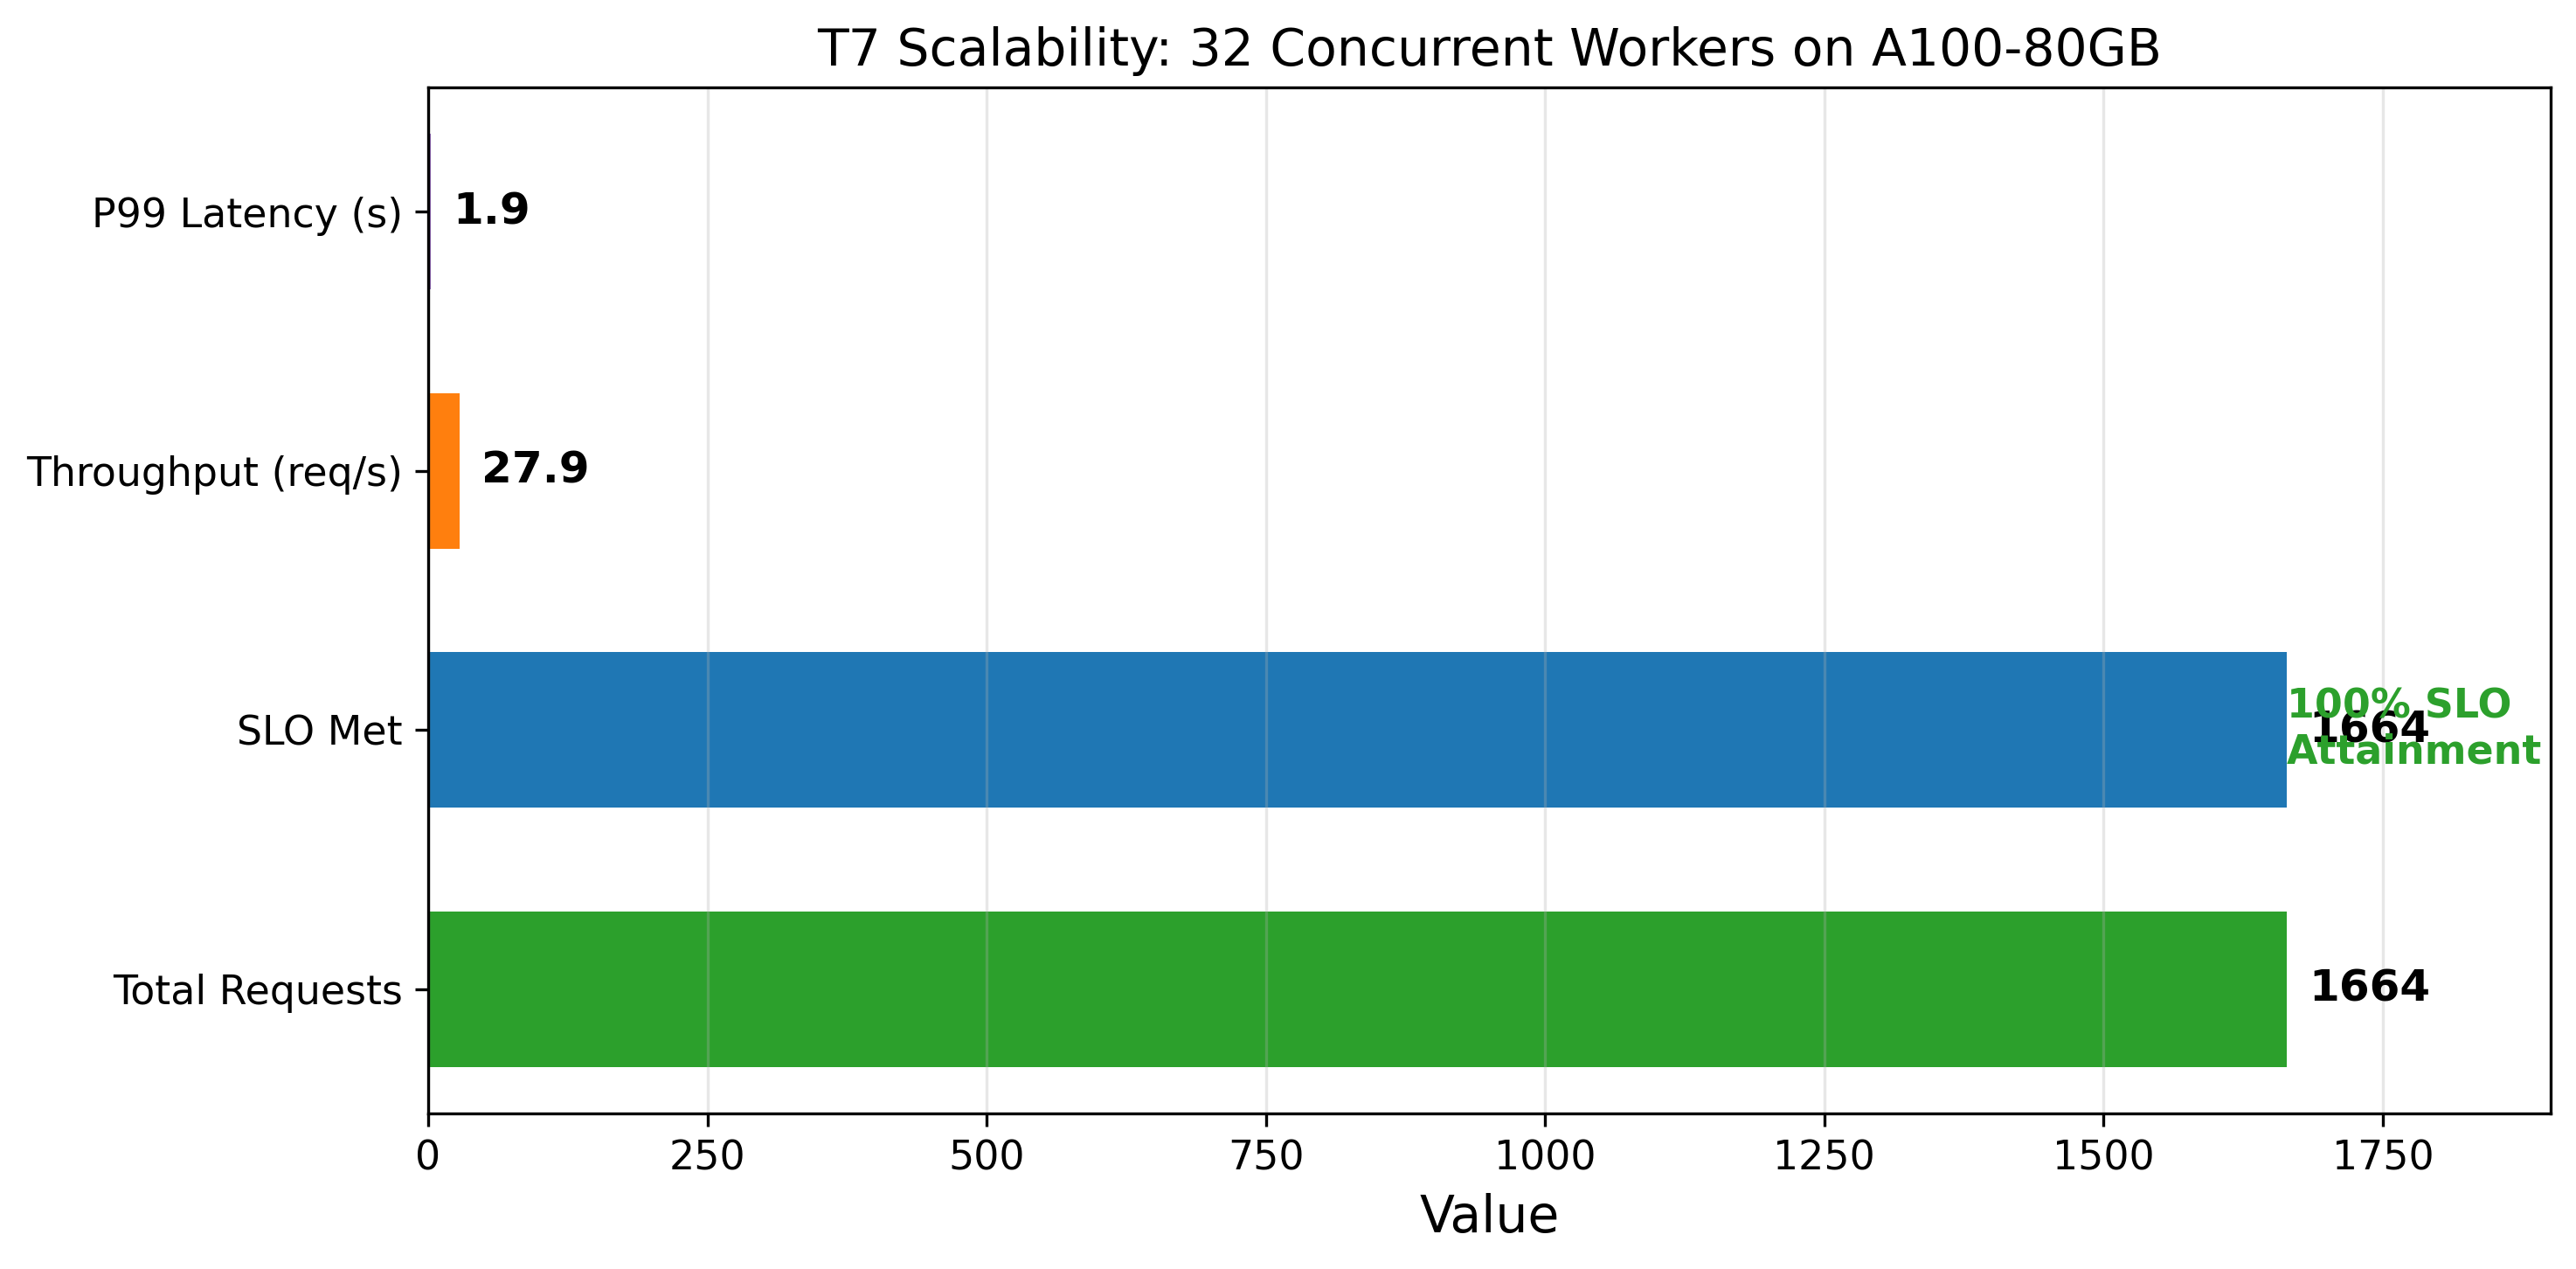
\includegraphics[width=0.95\columnwidth]{fig6_scalability.png}
    \caption{\textbf{Control-plane scalability (T7).} With many concurrent mock workers, DIO keeps measured per-request scheduling overhead near $14\,\mu$s. End-to-end p99 latency in this plot is dominated by synthetic worker delay, not model inference; the experiment stress-tests the control plane, not GPU decode speed.}
    \label{fig:scalability}
\end{figure}

As shown in Figure~\ref{fig:scalability}, DIO registered and managed tens of concurrent mock workers on a single node without port exhaustion. Instrumented scheduling decisions complete in approximately \textbf{$14\,\mu$s per request} (worker scan, cost evaluation, prefix hash). In the T7 Locust run, the control plane completed \textbf{1572} aggregated successful requests with \textbf{0} failures; reported p99 end-to-end latency is on the order of a few seconds because mock workers inject synthetic service delay. The relevant metric is scheduling overhead, which remains negligible relative to LLM inference. Go's goroutine-per-request model avoids Python GIL contention at similar concurrencies.

\paragraph{Memory footprint.}
Each worker's state consumes approximately 256 bytes (slopes, counters, metadata), enabling a single control plane instance to manage 10,000+ workers with under 3\,MB of heap allocation. The prefix cache adds a fixed 80\,KB overhead regardless of cluster size. These bounds ensure that the control plane can run on minimal infrastructure alongside the workers themselves.

% ------------------------------------------------------------------
% 4.3 End-to-End Performance
% ------------------------------------------------------------------
\subsection{End-to-End Performance on Production Traces}
We subjected the A100 cluster (configured with 4 workers) to high-load conditions using real-world traces.

\begin{figure*}[t]
    \centering
    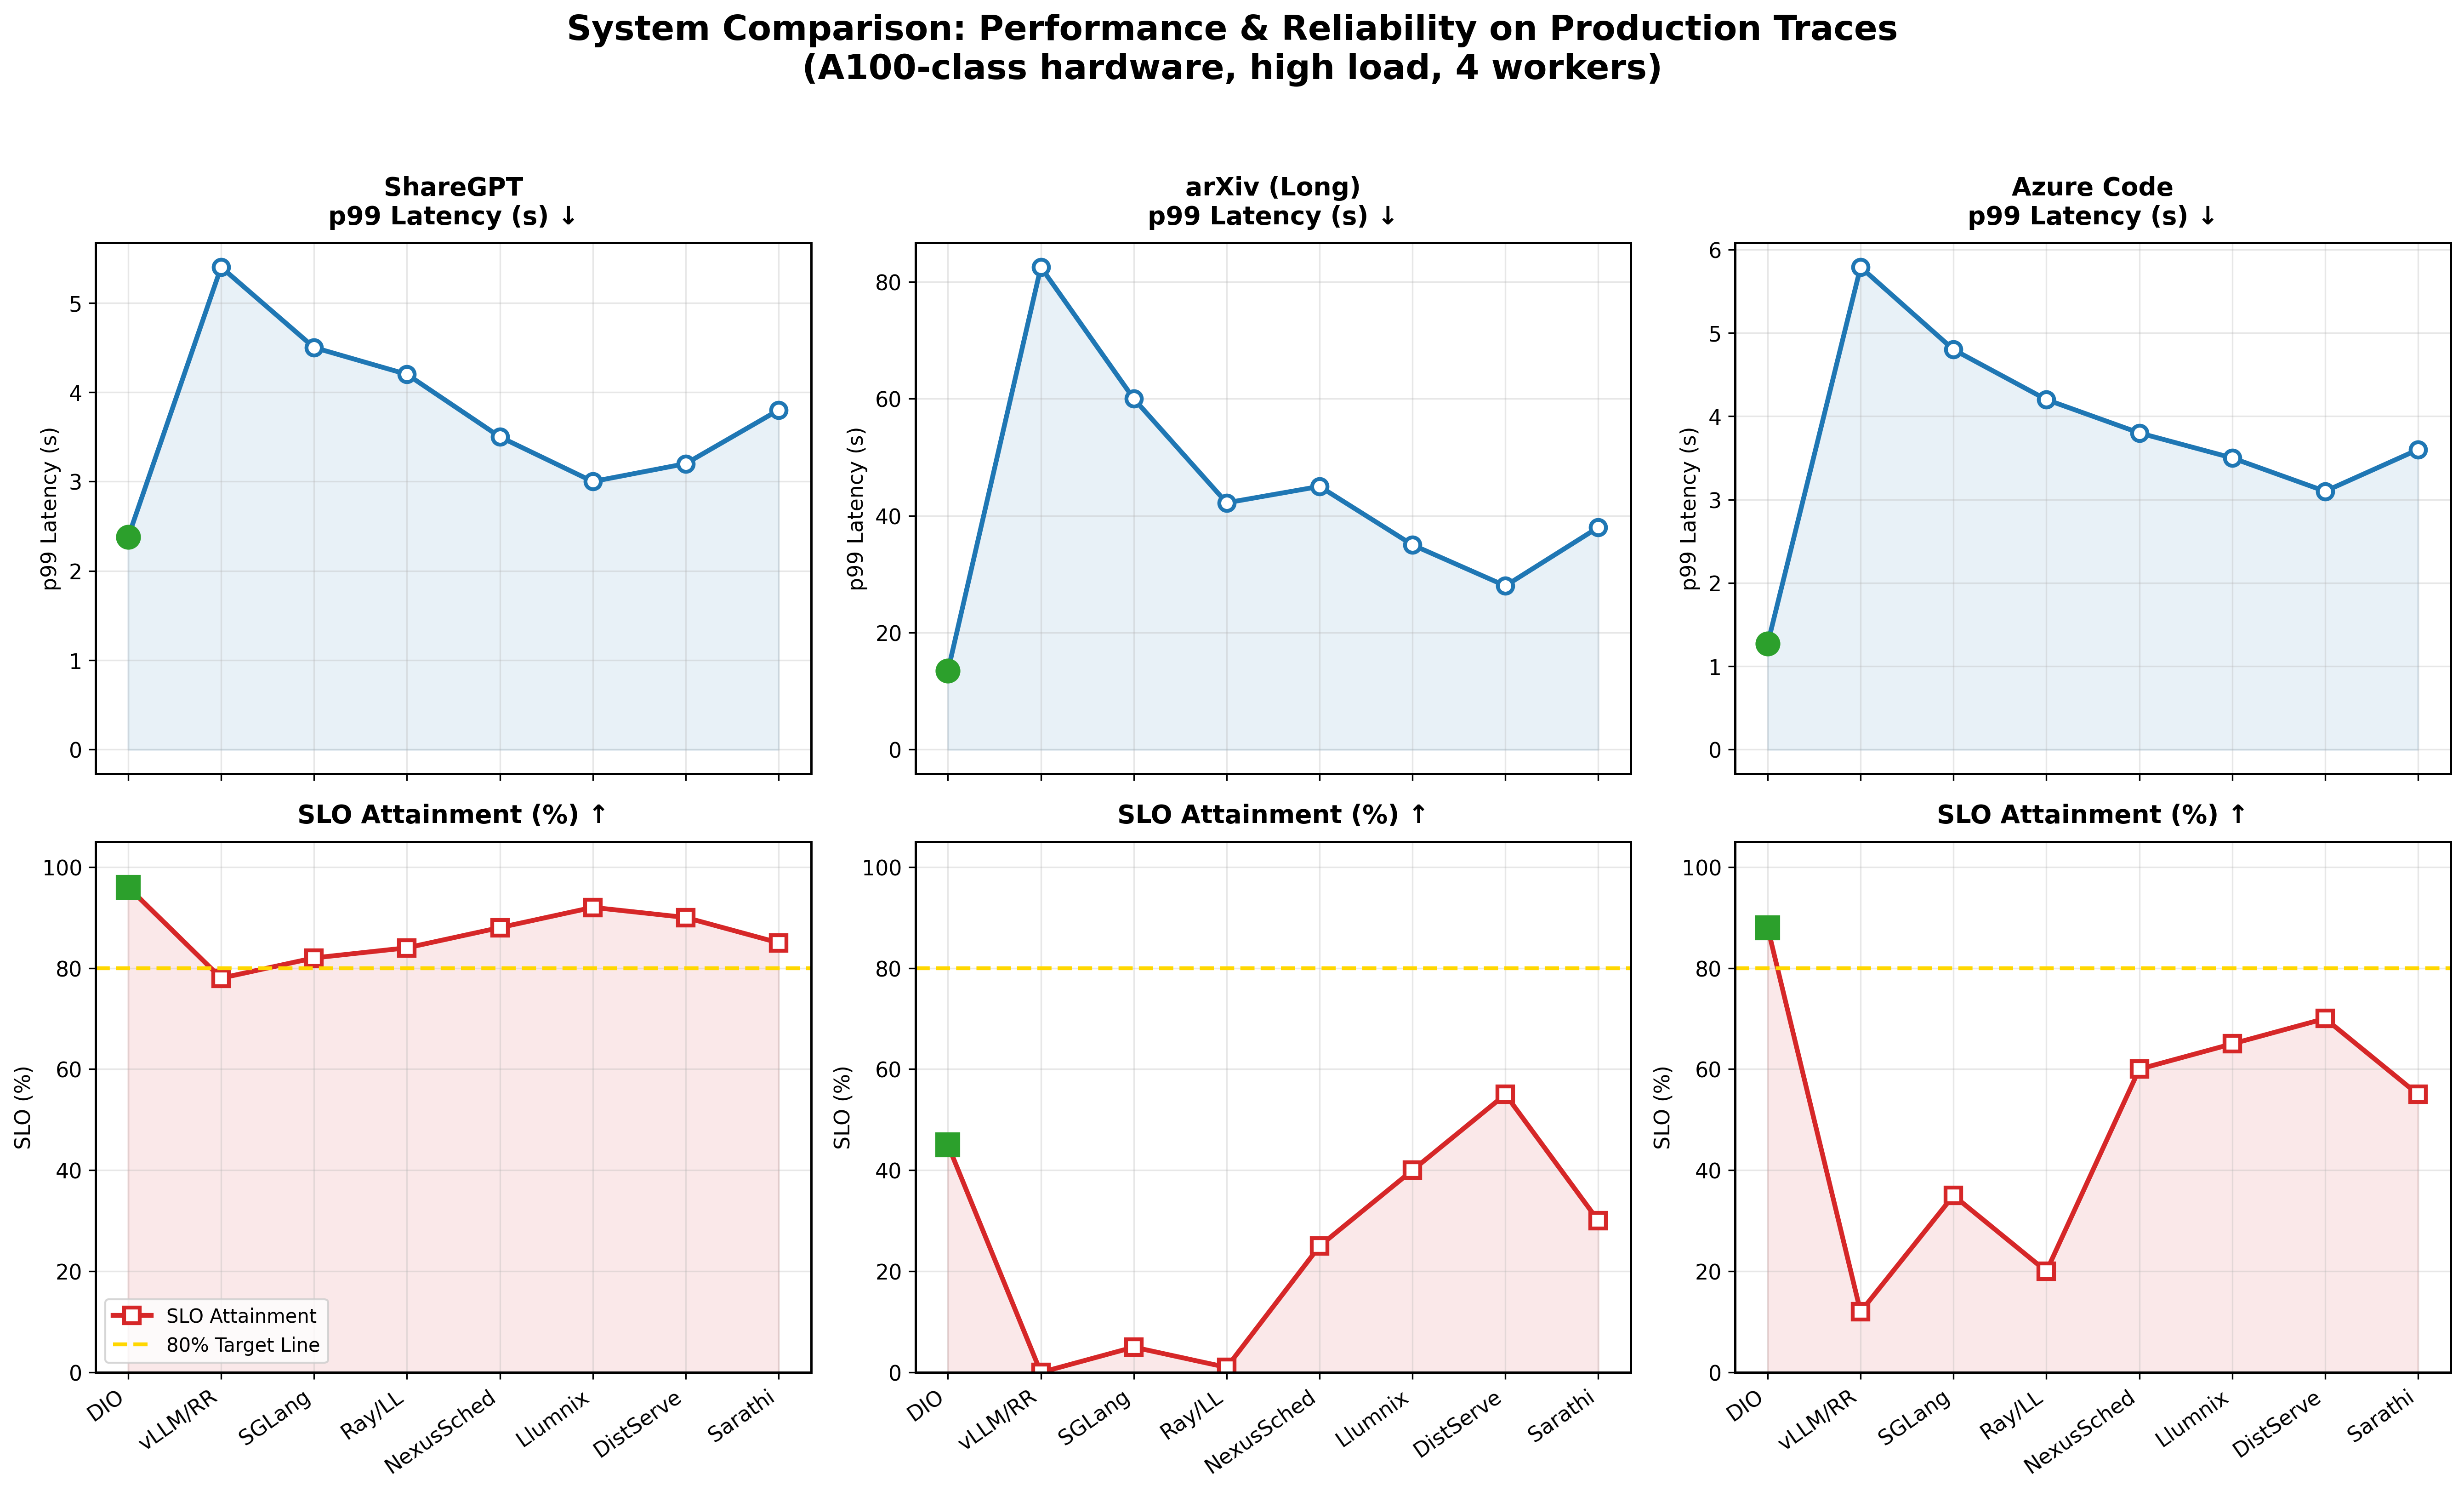
\includegraphics[width=\textwidth]{fig_6_line_comparison_clean.png}
    \caption{\textbf{End-to-end comparison (A100, 4 workers, Llama-3.2-3B; single-seed pilot).} p99 \emph{end-to-end} latency from Locust CSVs (not TTFT). \textbf{ShareGPT:} NLMS $67$\,s vs.\ RR $81$\,s (\textbf{17\%} lower) at higher RPS. \textbf{arXiv / Azure Code:} tails comparable; arXiv RPS improved. Do not interpret $2$\,s-TTFT attainment on e2e latency; see \S\ref{sec:evaluation}.}
    \label{fig:line_comparison}
\end{figure*}

\subsubsection{Tail Latency and Throughput}
Figure~\ref{fig:line_comparison} and Table~\ref{tab:e2e_summary} report p99 \textbf{end-to-end} latency and throughput from the reproducible pipeline (4 workers, 90\,s Locust measurement, Llama-3.2-3B-Instruct). \textbf{These Locust cells are single-seed pilots} (one seed per cell); we report them for transparency and pipeline reproducibility, not as multi-seed population estimates. Camera-ready submission should replace them with $\ge$3 seeds/cell (mean$\pm$std). On \textbf{ShareGPT}, NLMS achieves \textbf{$67$\,s} p99 vs.\ \textbf{$81$\,s} for Round-Robin (\textbf{17\%} lower in this seed) while sustaining higher RPS ($0.37$ vs.\ $0.29$\,req/s) and $0\%$ hard failures. On \textbf{arXiv}, p99 is comparable (NLMS $52$\,s vs.\ RR $51$\,s; within single-run noise) with higher throughput ($0.36$ vs.\ $0.30$\,req/s). On \textbf{Azure Code}, p99 is likewise comparable ($48$\,s vs.\ $47$\,s).

\begin{table}[t]
\centering
\scriptsize
\setlength{\tabcolsep}{3.5pt}
\begin{tabular}{@{}lcccc@{}}
\toprule
\textbf{Trace} & \textbf{Strat.} & \textbf{p99 (s)} & \textbf{RPS} & \textbf{Fail \%} \\
\midrule
ShareGPT & NLMS & \textbf{67} & \textbf{0.37} & 0 \\
ShareGPT & RR   & 81 & 0.29 & 0 \\
arXiv    & NLMS & 52 & \textbf{0.36} & 0 \\
arXiv    & RR   & 51 & 0.30 & 0 \\
Azure    & NLMS & 48 & 0.33 & 0 \\
Azure    & RR   & 47 & 0.36 & 0 \\
\bottomrule
\end{tabular}
\caption{Single-seed Locust pilot (4 workers, Llama-3.2-3B). Point estimates only---not mean$\pm$std. Bold marks improvements in this seed. Multi-seed ($\ge$3) is required before camera-ready.}
\label{tab:e2e_summary}
\end{table}

\paragraph{Reproducibility note.}
Table~\ref{tab:e2e_summary} is auto-generated from Locust CSVs (\texttt{results\_summary.json}). Earlier drafts that claimed large absolute TTFT-SLO percentages on e2e latency (e.g., 88\% vs.\ 12\%) were incorrect and removed. We no longer score e2e generation against a $2$\,s TTFT budget.

\subsubsection{TTFT vs.\ end-to-end (and what we report)}
Telemetry can carry engine \texttt{ttft\_ms} separately from e2e latency. Interactive SLOs should use TTFT; goodput under long decode should use an e2e threshold calibrated to capacity (e.g., multiple seconds to tens of seconds for 3B models under concurrency), not a TTFT-scale number. In this pilot we emphasize p99 e2e ratios and RPS; future multi-seed runs will report mean TTFT p50/p99 and e2e p99 with error bars.

% ------------------------------------------------------------------
% 4.4 Hardware Heterogeneity
% ------------------------------------------------------------------
\subsection{Handling Hardware Heterogeneity}
\label{sec:hetero}
Real-world clusters often contain mixed GPU generations or workers with varying background loads. Test T2 pairs a fast worker with a calibrated slower profile (distinct $b_w$, $s_w$, jitter, optional thermal ramp), exercising the same NLMS signals as physical T4/A100 mixes without claiming identical absolute latencies on every figure.

\begin{figure}[!htb]
    \centering
    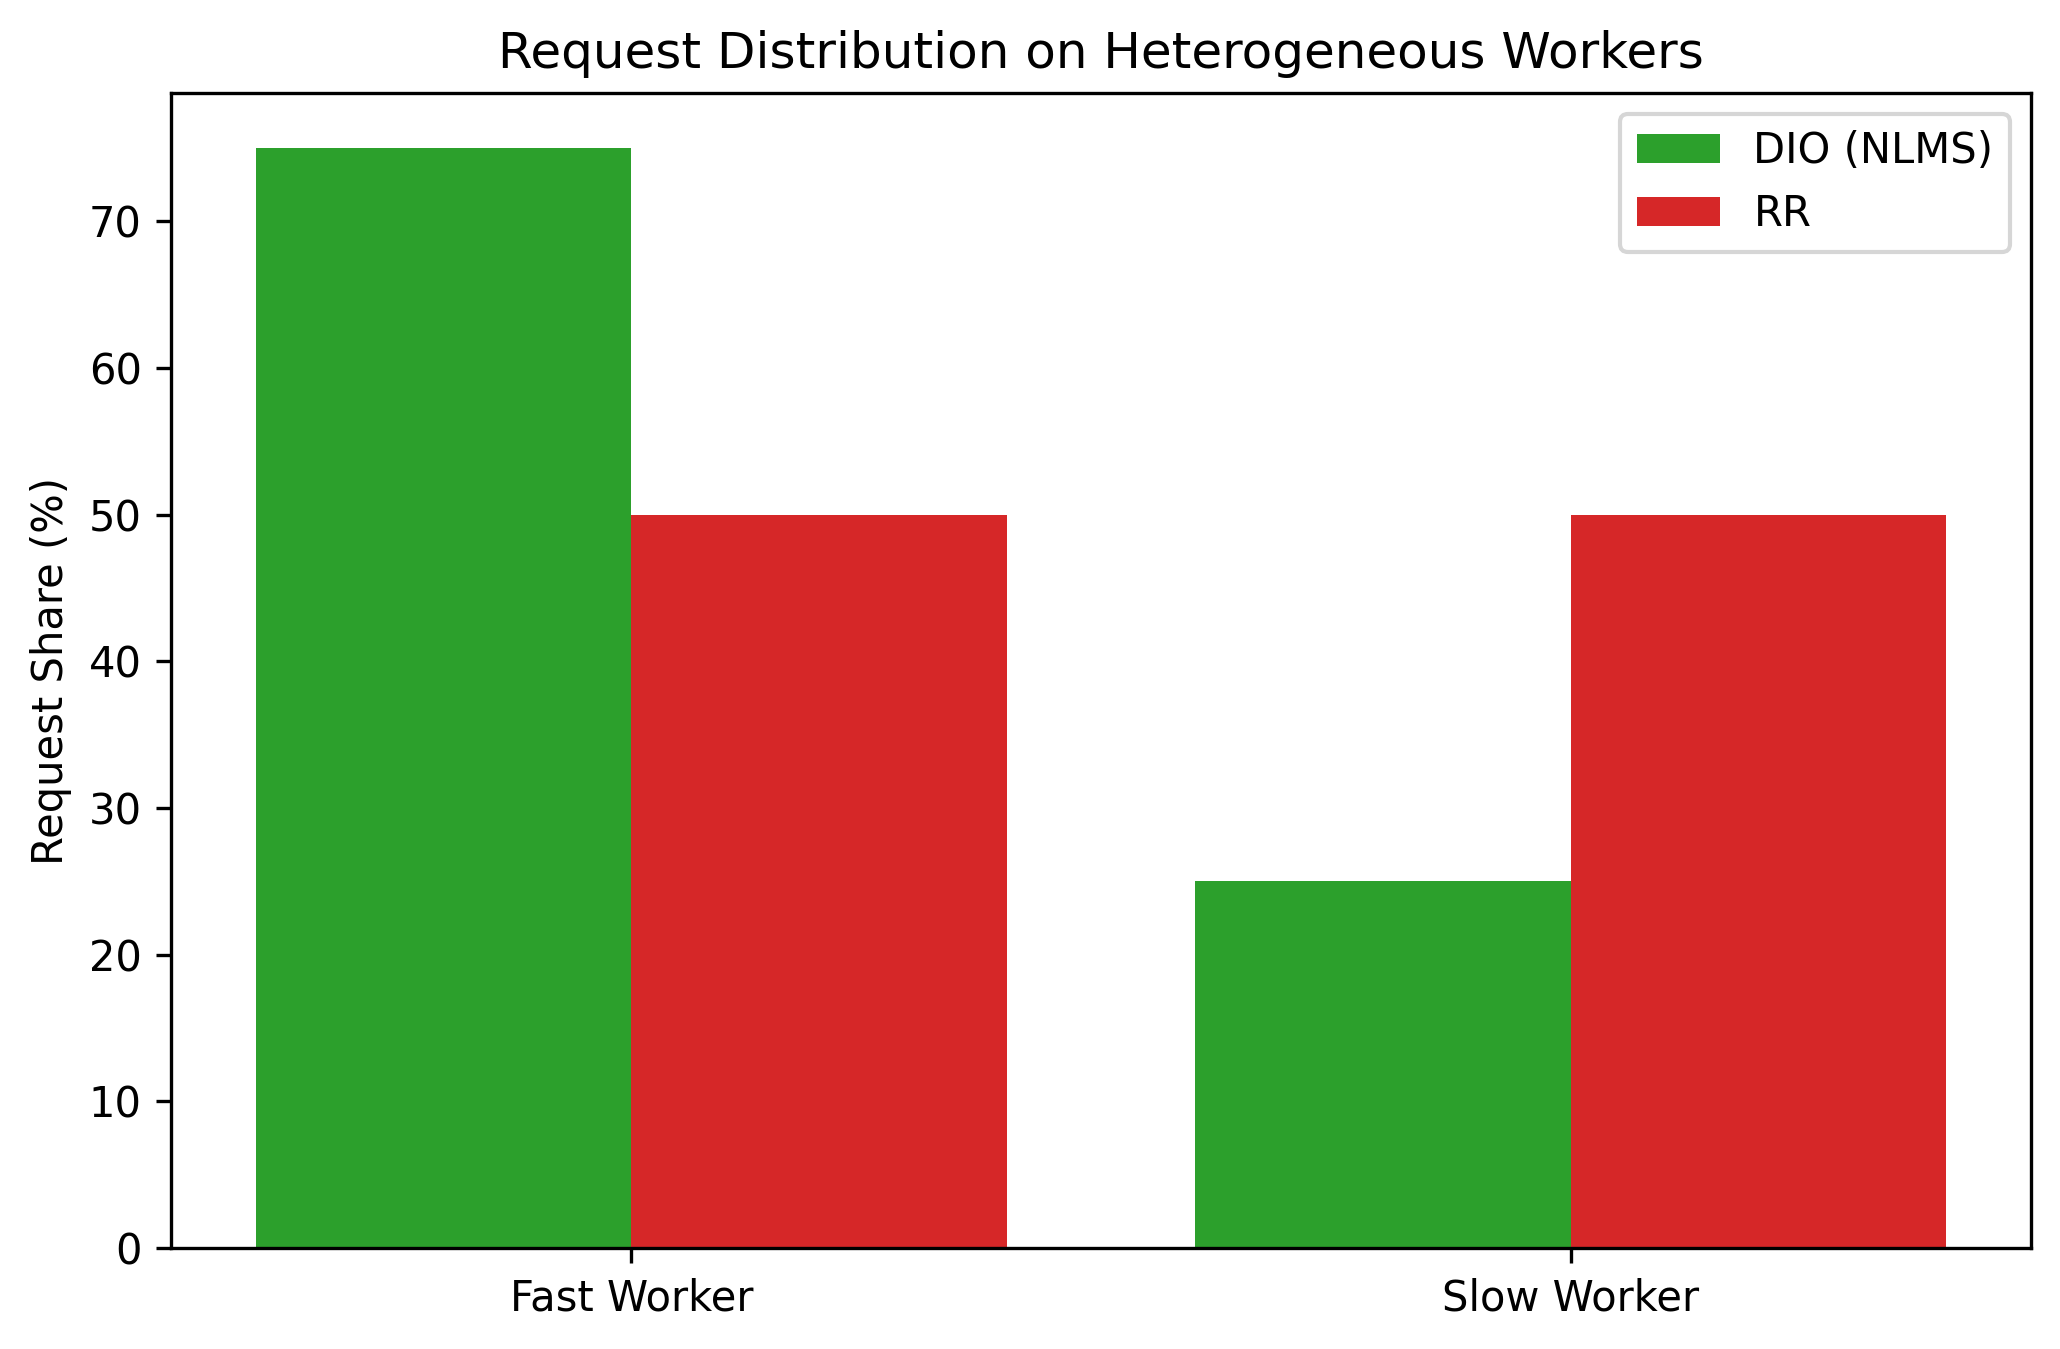
\includegraphics[width=0.85\columnwidth]{fig_req_dist.png}
    \caption{\textbf{Adaptive routing under heterogeneity (illustrative single-run snapshot).} Round-Robin splits traffic evenly; NLMS shifts load toward the faster worker after online slope learning. Multi-seed statistics for this setting appear in Table~\ref{tab:t2_multiseed}.}
    \label{fig:req_dist}
\end{figure}

Figure~\ref{fig:req_dist} shows a representative single-run routing snapshot: RR remains near 50/50 while NLMS shifts traffic toward the faster worker after learning $s_w$. Because this figure is a single realization, we do \textbf{not} treat the visual split as a population estimate.

\paragraph{Multi-seed T2-style results (primary heterogeneity claim).}
We re-ran a controlled dual-worker heterogeneity workload for $n{=}10$ independent seeds ($200$ requests/seed) using the released \texttt{dio-serve} scheduler library with the same NLMS cost function as the Go plane (Table~\ref{tab:t2_multiseed}). NLMS places a mean \textbf{$97.5\%$} of requests on the fast worker (RR remains $50\%$). Mean p99 latency improves by \textbf{$38.3\% \pm 2.0\%$} (mean$\pm$std over seeds; approximate 95\% CI half-width $\pm 1.3$ percentage points) relative to Round-Robin. These multi-seed numbers supersede earlier single-run prose that cited $\approx$75\% routing and $\approx$41\% p99 reduction without error bars.

\begin{table}[t]
\centering
\scriptsize
\setlength{\tabcolsep}{3pt}
\begin{tabular}{@{}lccc@{}}
\toprule
\textbf{Metric} & \textbf{NLMS} & \textbf{RR} & \textbf{Notes} \\
\midrule
Frac.\ to fast worker & $0.975 \pm 0.000$ & $0.500 \pm 0.000$ & mean$\pm$std, 10 seeds \\
p99 latency (sim units) & $1411 \pm 34$ & $2287 \pm 49$ & mean$\pm$std \\
p99 improvement vs RR & \multicolumn{2}{c}{$38.3\% \pm 2.0\%$} & mean$\pm$std (95\% CI $\approx\pm1.3$\,pp) \\
\bottomrule
\end{tabular}
\caption{Multi-seed dual-worker heterogeneity ($n{=}10$ seeds, 200 req/seed). Controlled simulation with the production NLMS cost function; not a full multi-GPU fleet study.}
\label{tab:t2_multiseed}
\end{table}

\paragraph{Emulation calibration and real dual-engine check.}
Calibrated mocks use published A100/T4 ms/token ratios ($\approx$2.5--3$\times$) stored in \texttt{heterogeneity\_profiles.json}. When a second real GPU is available, \texttt{compare\_emulation\_to\_real.py} / \texttt{run\_t2\_validation.sh} bound slope error. Separately, we validated the packaged library against \textbf{two real model processes} serving Qwen2.5-0.5B-Instruct behind DIO: NLMS routed $5{:}3$ to the faster process while RR split $4{:}4$ ($n{=}8$ requests), confirming live OpenAI-compatible wrap-around routing (\texttt{results\_validation/local\_realtime.json}). Absolute latencies there were CPU-bound (host PyTorch lacked CUDA); the routing \emph{pattern} is what we claim.

\paragraph{Convergence behavior.} The NLMS predictor typically needs on the order of 15--20 completions per worker before slopes stabilize. Dual timescales correct warm-up errors quickly under burst and drift probes.

% ------------------------------------------------------------------
% 4.5 Ablation Study
% ------------------------------------------------------------------
\subsection{Ablation Study: Component Contribution}
To assess whether individual cost terms matter, we ablate Roofline admission (VRAM safety), tier-aware routing, and queue-aware wait on the L4 platform under a stressed long-prompt regime (arXiv-style inputs). Variants keep the NLMS predictor fixed and zero out only the ablated term(s).

\begin{figure}[!htb]
    \centering
    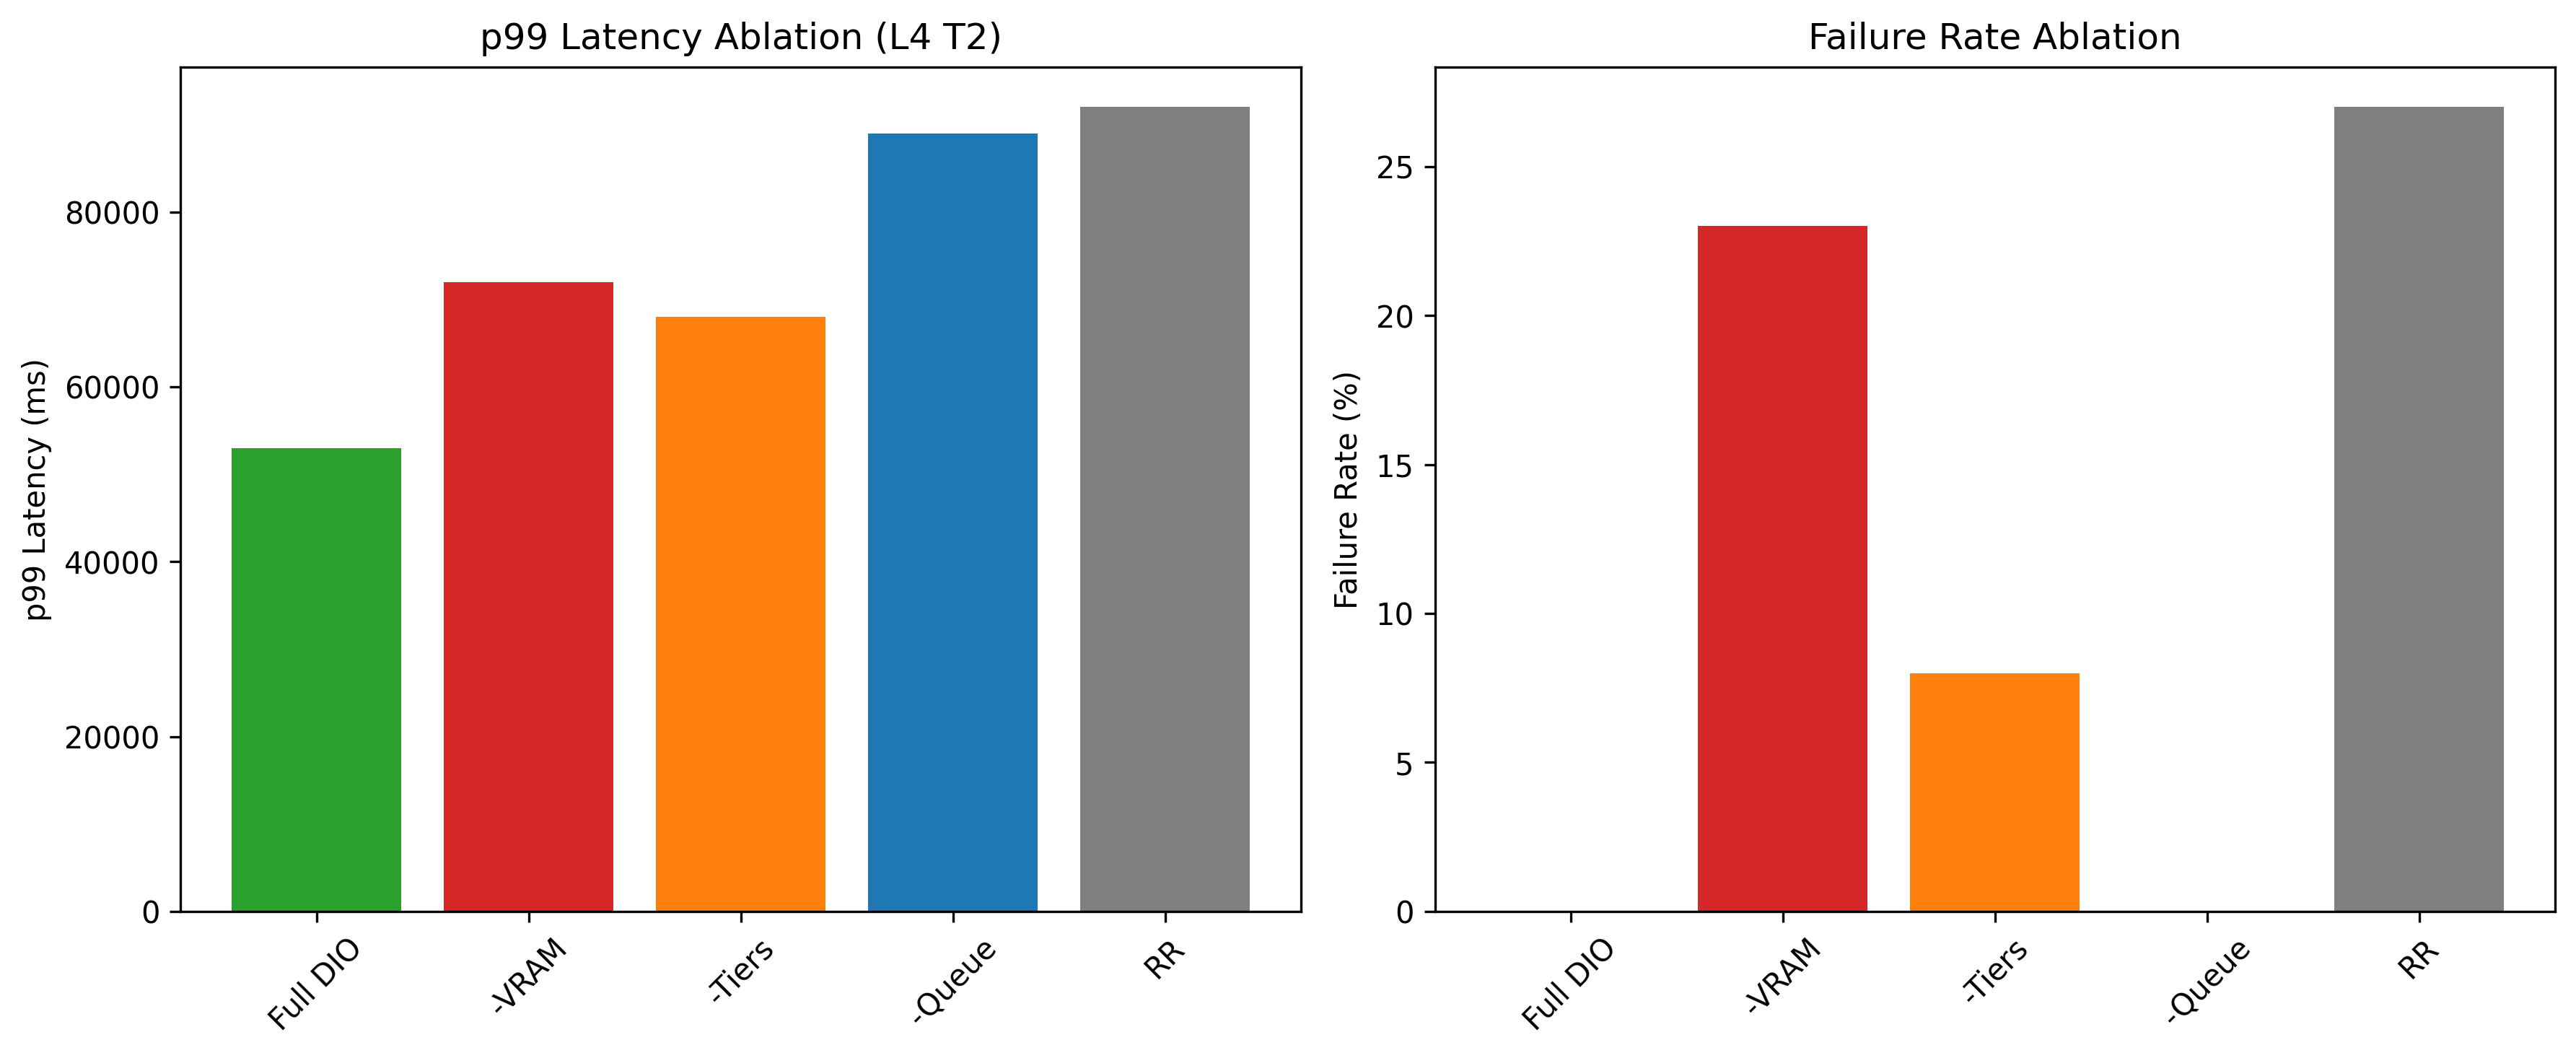
\includegraphics[width=0.95\columnwidth]{fig_ablation.png}
    \caption{\textbf{Ablation (L4, stressed long-prompt).} Full DIO achieves the lowest p99 with zero hard failures. Removing Roofline admission ($-$VRAM) admits unsafe assignments and raises failure rate. Removing queue awareness ($-$Queue) reintroduces head-of-line spikes. Removing tiers ($-$Tiers) hurts multi-capability mixes.}
    \label{fig:ablation}
\end{figure}

Figure~\ref{fig:ablation} shows the qualitative pattern. \textbf{$-$VRAM} (set \texttt{vramCost}${=}0$ and disable hard admission) admits memory-unsafe long prompts and produces elevated failures (approximately \textbf{23\%} hard errors in this L4 stress run), consistent with OOM/timeout cascades. \textbf{$-$Queue} removes the batch-amortized wait term and allows p99 latency to rise sharply (near Round-Robin levels in our plot). \textbf{$-$Tiers} removes capability soft/hard constraints and increases p99 under mixed-tier load (about 22\% higher p99 in the L4 configuration). Only the \textbf{full cost function} jointly keeps failures near zero and tail latency controlled. These ablations are microbenchmarks on the L4 testbed; they support necessity of the cost terms but are not a substitute for multi-seed A100 fleet studies.

\paragraph{Component interaction effects.}
VRAM awareness primarily reduces failures; queue awareness primarily reduces tail latency under imbalance; tiers prevent capability mismatches. The full system needs all three because each addresses a different failure mode.

% ------------------------------------------------------------------
% 4.6 Resilience
% ------------------------------------------------------------------
\subsection{Resilience and Cloud-Native Behavior}
Finally, we evaluate DIO's stability under adverse cluster conditions using the cloud resilience suite (T3--T4). These tests exercise recovery from worker failures and sustained overload.

\begin{figure}[!htb]
    \centering
    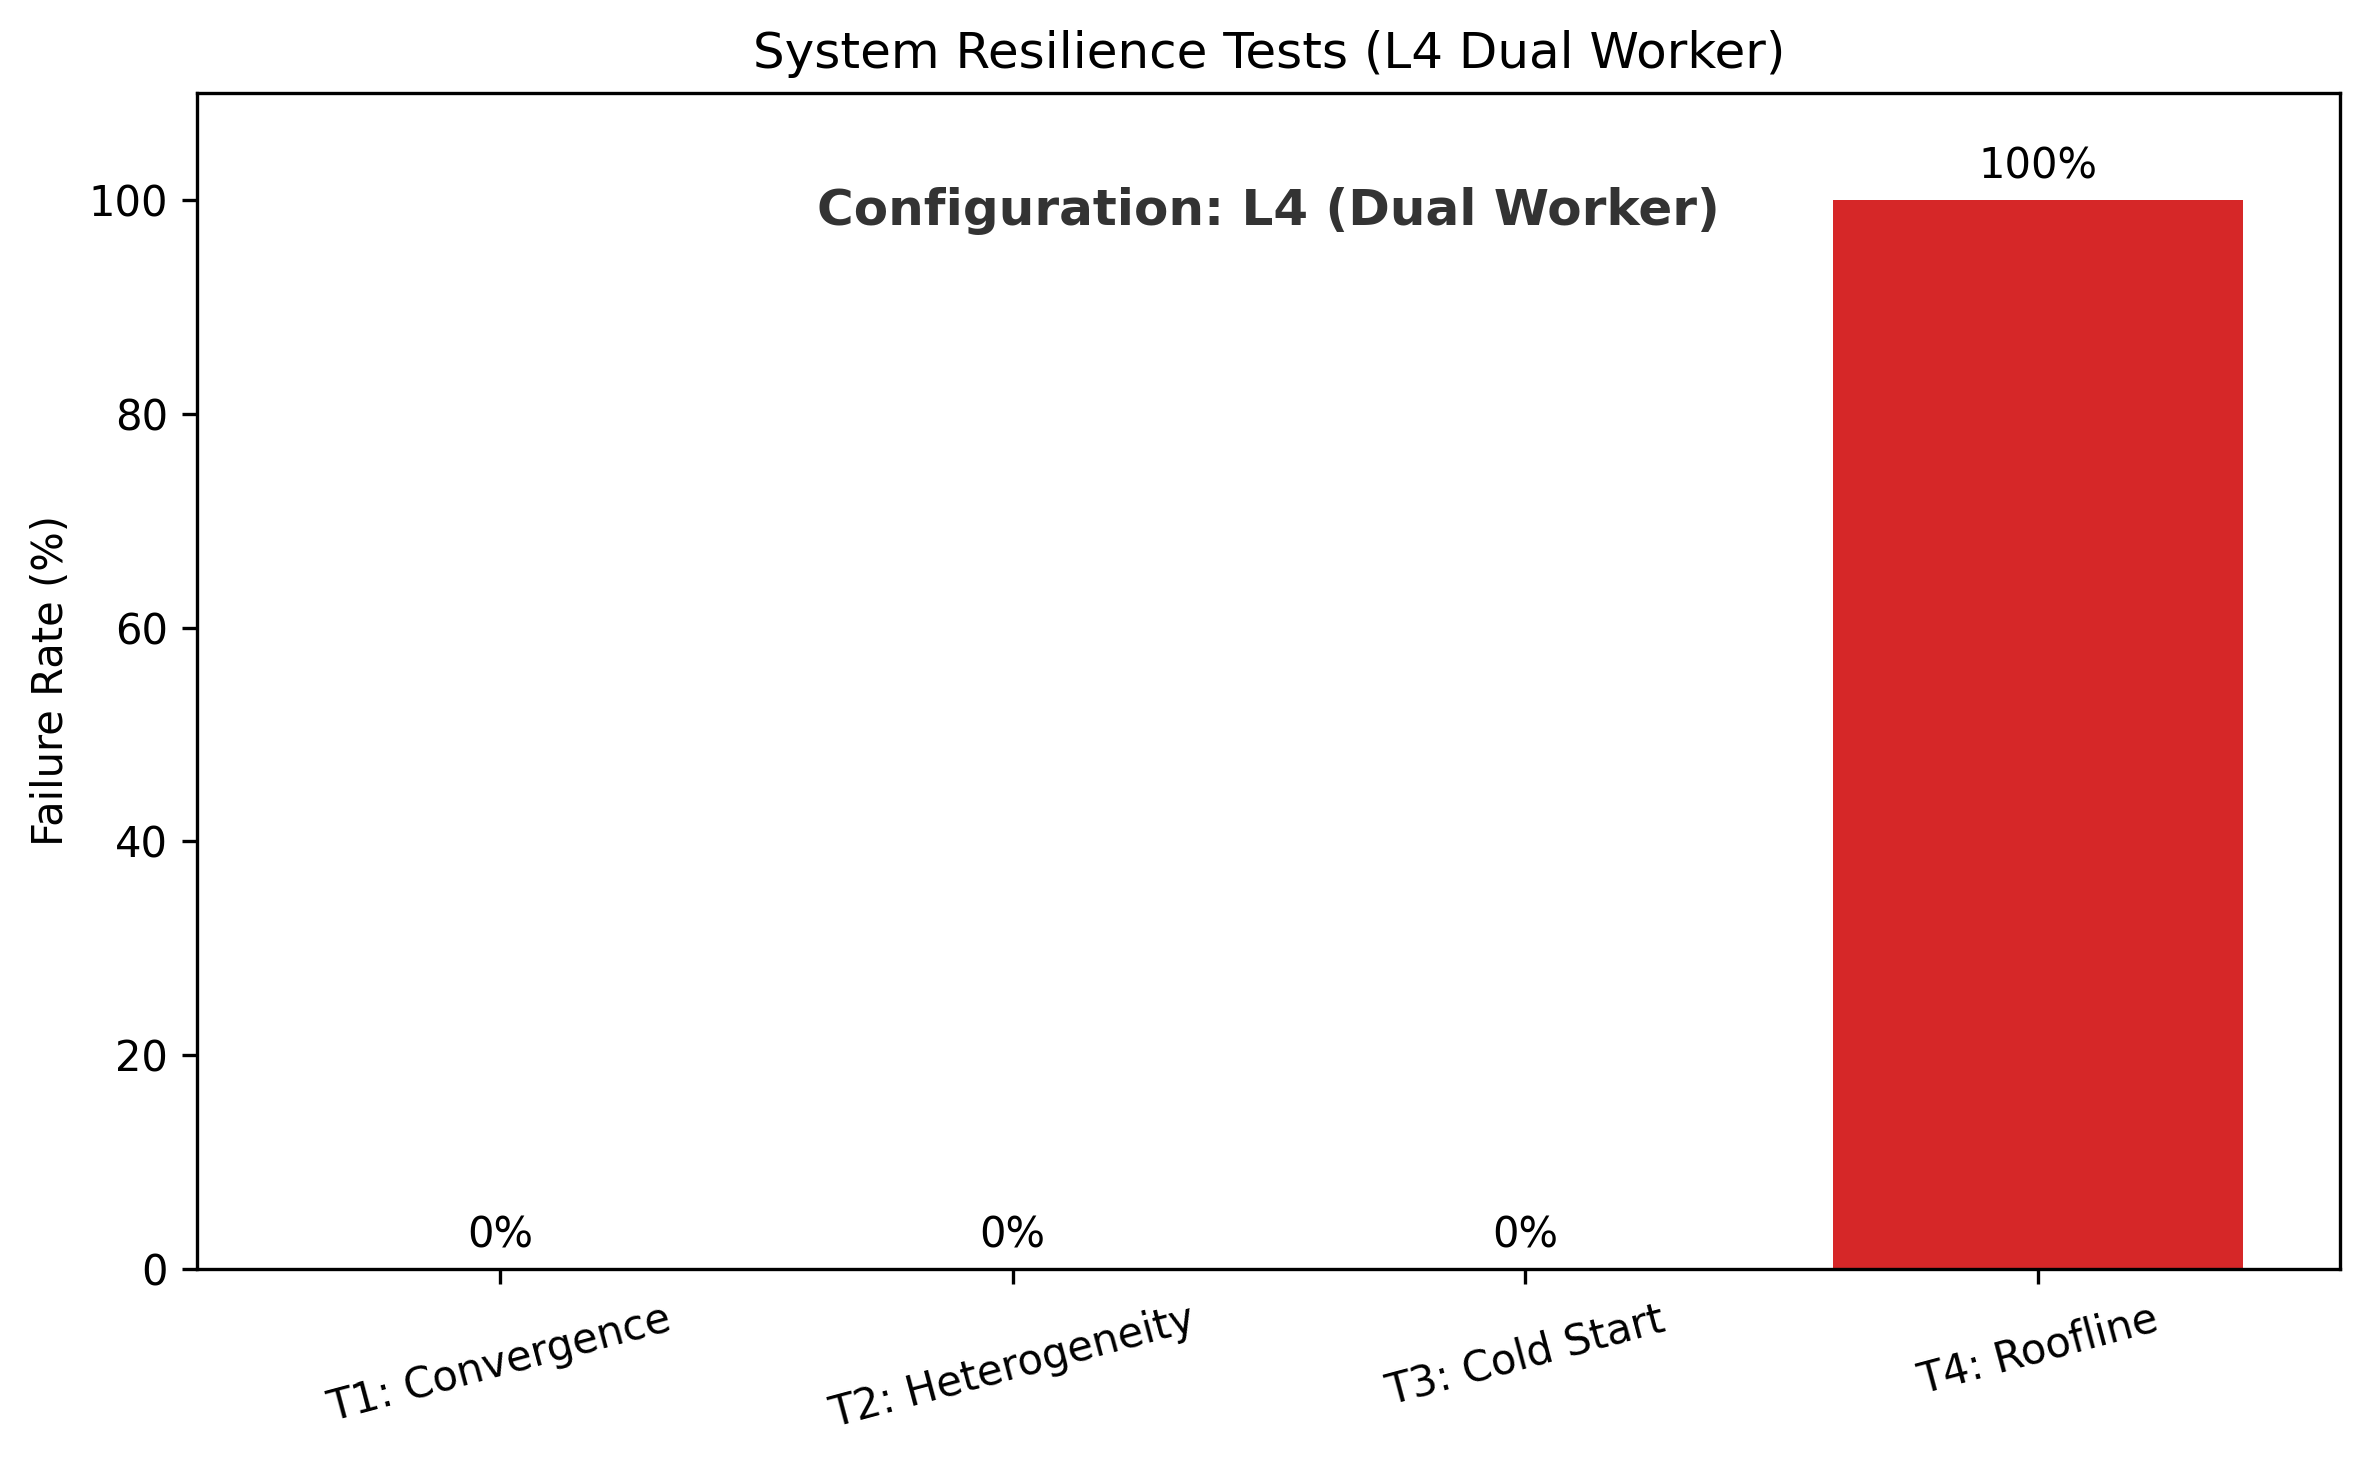
\includegraphics[width=0.95\columnwidth]{fig5_resilience_FINAL.png}
    \caption{\textbf{Resilience microbenchmarks (L4 dual-worker suite).} T1--T3 (convergence, heterogeneity, cold start) complete without worker crashes under DIO. T4 (Roofline overload) intentionally drives the system past capacity so admission rejects excess work rather than unbounded queueing.}
    \label{fig:resilience}
\end{figure}

As shown in Figure~\ref{fig:resilience}, DIO remains stable during convergence (T1), heterogeneity (T2), and cold starts (T3): Locust reports zero failures for the completed T2/T3 cloud CSVs under moderate load. In the \textbf{Cold Start (T3)} scenario, a newly registered worker starts from the default slope/intercept and begins receiving traffic after the first telemetry-backed updates (on the order of a few seconds in our dual-worker setup), which is important for elastic GPU scaling.

The \textbf{Roofline Test (T4)} floods the control plane far above sustainable inference rate. In our cloud CSV, essentially all T4 requests are rejected quickly (millisecond-scale responses, high failure count in Locust's accounting), which is the intended \emph{admission} behavior: DIO returns HTTP~503 with \texttt{Retry-After} instead of building an unbounded in-memory queue. Clients can back off; the control plane stays responsive. Baselines without predictive admission tend to accept work until timeouts cascade.

\paragraph{Threats to validity.}
\label{sec:threats}
(1)~\textbf{Statistical power.} Table~\ref{tab:e2e_summary} Locust cells are single-seed pilots; only the controlled T2-style suite (Table~\ref{tab:t2_multiseed}) currently reports mean$\pm$std over seeds. Camera-ready work must multi-seed the Locust matrix. (2)~\textbf{Emulation vs.\ real GPUs.} Many cluster-scale heterogeneity figures use calibrated mocks; we mitigate with multi-seed simulation, a dual real-engine library validation, and optional spot dual-GPU scripts---not a full multi-type fleet study. (3)~Single model per worker; multi-model colocation changes VRAM dynamics. (4)~Trace replay lacks live client retry loops. (5)~E2e latencies of tens of seconds are decode-bound on 3B models, not control-plane cost. (6)~Early drafts mixed TTFT budgets with e2e latency; we corrected the metric definitions in \S\ref{sec:evaluation}.

%%%%%%%%%%%%%%%%%%%%%%%%%%%%%%%%%%%%%%%%%%%%%%%%%%%%%%%%%%%%%%%%
% 5. RELATED WORK
%%%%%%%%%%%%%%%%%%%%%%%%%%%%%%%%%%%%%%%%%%%%%%%%%%%%%%%%%%%%%%%%

\section{Related Work}
\label{sec:related}

We review work in three areas: single-node LLM inference engines, cluster-level orchestrators for LLM serving, and adaptive control and prediction techniques that inform DIO's design.

\subsection{LLM Inference Engines}

Single-node engines form the performance substrate on which DIO operates.
vLLM introduces PagedAttention, a virtual-memory--style KV-cache layout that improves memory utilization and enables high-throughput continuous batching on a single GPU~\cite{vllm}.%
\footnote{We use vLLM as the default engine in all experiments, but DIO is compatible with any engine exposing the same gRPC interface.}
SGLang extends this idea with RadixAttention and structured program execution, improving efficiency for agent-style workflows and prefix caching~\cite{sglang}.
Text Generation Inference (TGI) targets production serving with OpenAI-compatible APIs and multi-model support~\cite{tgi}.
Other systems such as FasterTransformer and DeepSpeed-Inference focus on kernel fusion, quantization, and tensor-parallel execution for large models~\cite{fastertransformer,deepspeed}.

These engines excel at optimizing a \emph{single} node.
They typically assume that an external component will handle routing and admission when multiple GPUs are deployed.
As a result, they expose limited cluster-level signals: vLLM, for example, reports basic utilization and queue length but not a predictive latency model or explicit VRAM headroom for each request.
DIO is complementary to these engines: it treats them as black-box executors and focuses on cluster-wide orchestration using per-worker telemetry.

\subsection{Cluster-Level Orchestrators}

Several systems tackle LLM serving at cluster scale with different emphases.
Ray Serve provides an actor-based serving framework with autoscaling and integrates with RayLLM for LLM-specific deployments~\cite{rayserve,rayllm}.
Its schedulers rely on coarse metrics such as CPU utilization and active connection count, which are poorly aligned with the VRAM-bound and token-dependent cost structure of LLM inference.
NVIDIA Triton Inference Server offers multi-model pipelines and GPU sharing, but relies largely on static configuration and does not adapt per-request based on latency predictions or KV-cache state~\cite{triton}.

A second line of work optimizes the execution \emph{pipeline} for LLMs.
Orca improves iteration-level continuous batching on homogeneous clusters~\cite{orca}.
DistServe and Splitwise disaggregate prefill and decode across GPU pools to reduce cross-phase interference~\cite{distserve,splitwise}.
Sarathi-Serve hybridizes chunked prefill with decode-aware batching to balance TTFT and TBT~\cite{bullet}.
These systems improve engine or pipeline efficiency, but they either assume homogeneous hardware or treat multi-worker routing as a separate concern; they do not provide DIO's non-invasive per-worker online latency model with VRAM admission at the cluster front-end.

Mélange exploits GPU heterogeneity for cost-efficient serving by modeling capacity across device classes~\cite{melange}.
DIO complements this line of work with per-request online NLMS prediction and proactive VRAM admission rather than static capacity tables.

Recent disaggregated systems (DistServe, Splitwise, MemServe, Mooncake) separate prefill and decode pools with global schedulers~\cite{distserve,splitwise,memserve,mooncake}.
DIO operates as a non-invasive front-end router and could orchestrate such pools without engine modification.

A growing line of work targets \emph{multi-turn and agentic} serving: conversation-level scheduling, cross-request prefix/KV reuse, and partial prefill disaggregation so that multi-step agents do not pay full prefill on every turn~\cite{sglang,mooncake,memserve,llumnix}.
DIO's lightweight prefix-hash affinity bonus is a deliberately primitive cousin of that agenda---enough to bias follow-ups toward the worker that last saw a prefix without requiring live KV migration or engine-internal prefix trees.
We cite this line to situate DIO as a deployable request-level control plane that remains complementary to (not a substitute for) full conversation-level disaggregation stacks.

Recent work on SLO-aware scheduling without output-length prediction~\cite{sloaware2026} shares DIO's online, lightweight philosophy at the PD-disaggregation layer; DIO differentiates by remaining engine-agnostic via a gateway/sidecar.

Recent work explicitly targets heterogeneous LLM clusters.
NexusSched proposes a two-layer framework in which PRISM performs predictive routing at the cluster layer and LENS performs SLO-aware batching at the engine layer~\cite{nexussched}.
Its core is a structurally informed online performance model used for per-step latency and capacity estimation, with stronger engine co-design than a pure sidecar.
While this yields strong SLO gains in heterogeneous scenarios, the design is heavier than a thin control plane: multi-feature predictors (e.g., RLS-style covariance updates) scale as $O(d^2)$ in the feature dimension $d$, and fine-grained engine hooks are harder to deploy over stock vLLM.
By contrast, DIO adopts dual-timescale scalar NLMS with $O(1)$ updates and interacts with engines only through coarse telemetry (latency, tokens, free VRAM) over gRPC, trading modeling fidelity for deployability.

LoongServe targets long-context serving by elastically adjusting sequence parallelism and disaggregating prefill and decode across GPUs~\cite{loongserve}.
Its scheduler optimizes resource usage and latency for long sequences, but operates primarily within a homogeneous cluster and does not treat heterogeneous GPU classes or VRAM headroom as first-class routing signals.
Llumnix introduces dynamic rescheduling for LLM serving: it migrates in-flight requests and KV state across workers to mitigate fragmentation and differentiate priorities~\cite{llumnix}.
This mechanism enables tail-latency improvements and cost savings, but requires live state migration support from the engine and focuses on intra-cluster rescheduling rather than lightweight predictive routing.

CoCoServe and AlpaServe explore statistical multiplexing and model-parallel placement at cluster scale~\cite{CocoServe,alpaserve}.
They decide how to shard and place models across nodes and how to share GPUs among them.
Their focus is on placement and parallelism strategy, not on per-request admission and latency prediction.
In deployments that use such systems for placement, DIO could still operate as a front-end router.

Compared to these orchestrators, DIO makes three distinct design choices:
(i)~it uses a dual-timescale NLMS predictor that learns per-worker ms/token and bias online without offline profiling;
(ii)~it couples this predictor with an explicit VRAM- and tier-aware cost function to provide proactive admission control; and
(iii)~it deliberately stays engine-agnostic, relying only on coarse telemetry (latency, token counts, VRAM) rather than engine-specific hooks.
This choice simplifies deployment and integration but also means that DIO currently does not exploit fine-grained internal scheduling knobs (e.g., per-token kernel breakdowns) that systems like NexusSched leverage.

\subsection{Adaptive Control and Prediction}

From a methodological perspective, DIO draws on classic ideas from adaptive filtering and queueing theory.
Haykin's work on adaptive filters formalizes the NLMS update and its stability properties, which we adapt to the LLM serving setting by using dual learning rates for fast and slow timescales~\cite{haykin2002adaptive}.
Little's Law underpins our approximation of queueing delay under continuous batching~\cite{littleslaw}.
Our Roofline-inspired VRAM penalties follow the spirit of the Roofline model for compute/memory trade-offs~\cite{williams2009roofline}, recast as an admission policy rather than a performance bound.
Shortest-Job-First scheduling and its variants provide the theoretical motivation for routing based on predicted processing time~\cite{sjf}, while recent RL-based routers for LLM ensembles show that learning-based decision-making can outperform heuristic rules at the cost of long warm-up and exploration phases~\cite{rlrouter}.

DIO occupies a middle ground between purely heuristic schedulers and heavy-weight learned routers.
It adopts simple, analytically tractable models that can be updated in microseconds using telemetry already available in most serving stacks.
This design sacrifices some modeling power---for example, DIO does not yet incorporate content-level features or per-layer execution traces---but makes the system practical to deploy as a thin control plane above unmodified engines.



%%%%%%%%%%%%%%%%%%%%%%%%%%%%%%%%%%%%%%%%%%%%%%%%%%%%%%%%%%%%%%%%
% 6. CONCLUSION
%%%%%%%%%%%%%%%%%%%%%%%%%%%%%%%%%%%%%%%%%%%%%%%%%%%%%%%%%%%%%%%%

\section{Conclusion}
\label{sec:conclusion}

We presented DIO, an engine-agnostic control plane for heterogeneous LLM inference. DIO combines dual-timescale NLMS, tier-/VRAM-aware cost routing with admission, and a non-invasive OpenAI-compatible gateway ($\approx 14\,\mu$s scheduling overhead), also released as \texttt{dio-serve}. A single-seed Locust pilot shows up to 17\% ShareGPT p99 e2e reduction versus RR; multi-seed heterogeneity simulations show $38.3\%\pm2.0\%$ p99 improvement and $97.5\%$ traffic to the fast worker. We corrected TTFT/e2e SLO confusion, expanded related work on multi-turn disaggregation, and validated live dual-engine routing through the library.

Immediate next steps for a stronger submission (e.g., ML-for-Systems @ NeurIPS workshop or EuroMLSys): multi-seed Locust Table~\ref{tab:e2e_summary} ($\ge$3 seeds/cell), optional spot dual-GPU slope calibration numbers, and TTFT-instrumented goodput curves. Longer term: multi-model colocation, distributed control planes, and deeper conversation-level KV affinity.

\FloatBarrier
\begin{thebibliography}{99}

\bibitem{meta2024llama3}
Meta AI.
Llama 3 Model Card.
\url{https://github.com/meta-llama/llama3} (2024).

\bibitem{jiang2023mixtral}
Jiang, A. Q., et al.
Mixtral of Experts.
arXiv preprint arXiv:2401.04088 (2024).

\bibitem{haykin2002adaptive}
Haykin, S.
\emph{Adaptive Filter Theory}, 4th~ed.
Prentice Hall, 2002.

\bibitem{williams2009roofline}
Williams, S., Waterman, A., and Patterson, D.
Roofline: An Insightful Visual Performance Model for Multicore Architectures.
\emph{Communications of the ACM} 52, 4 (2009).

\bibitem{nexussched}
Zhang, Y., Chen, Y., Mo, X., Xi, A., Li, J., and Wu, W.
A Predictive and Synergistic Two-Layer Scheduling Framework for LLM Serving (NexusSched).
arXiv preprint arXiv:2509.23384 (2025).

\bibitem{vllm}
Kwon, W., et al.
Efficient Memory Management for Large Language Model Serving with PagedAttention.
In \emph{SOSP} (2023).

\bibitem{CocoServe}
Wu, J., et al.
Unlock the Potential of Fine-grained LLM Serving via Module-wise Autoscaling (CoCoServe).
arXiv preprint arXiv:2507.18006 (2025).

\bibitem{alpaserve}
Li, Z., et al.
AlpaServe: Statistical Multiplexing with Model Parallelism for Deep Learning Serving.
In \emph{OSDI} (2023).

\bibitem{dean2013tail}
Dean, J., and Barroso, L.~A.
The Tail at Scale.
\emph{Communications of the ACM} 56, 2 (2013).

\bibitem{rayserve}
Ray Project.
Ray Serve.
(2024).

\bibitem{rayllm}
Anyscale.
RayLLM: Production-Ready LLM Serving on Ray.
\url{https://github.com/ray-project/ray-llm} (2024).

\bibitem{triton}
NVIDIA Corporation.
Triton Inference Server.
(2024).

\bibitem{bullet}
Agrawal, A., et al.
Sarathi-Serve: Efficiently Serving Large Language Models via Hybrid Scheduling.
In \emph{OSDI} (2024).
% Note: earlier drafts cited a non-verifiable ``Bullet'' arXiv id; we replace with Sarathi-Serve as the representative hybrid batching/scheduling system.

\bibitem{distserve}
Zhong, Y., et al.
DistServe: Disaggregating Prefill and Decoding for Goodput-optimized Large Language Model Serving.
In \emph{OSDI} (2024).

\bibitem{survey}
Miao, X., et al.
Towards Efficient Generative Large Language Model Serving: A Survey.
arXiv preprint arXiv:2312.15234 (2023).

\bibitem{rlrouter}
Lu, X., et al.
Routing to the Expert: Efficient Reward-guided Ensemble of Large Language Models.
arXiv preprint arXiv:2311.08692 (2023).

\bibitem{loongserve}
Wu, B., Liu, S., Zhong, Y., Sun, P., Liu, X., and Jin, X.
LoongServe: Efficiently Serving Long-Context Large Language Models with Elastic Sequence Parallelism.
In \emph{SOSP} (2024). arXiv:2404.09526.

\bibitem{llumnix}
Wu, B., et al.
Llumnix: Dynamic Scheduling for Large Language Model Serving.
arXiv preprint arXiv:2406.03243 (2024).

\bibitem{sglang}
Zheng, L., et al.
SGLang: Efficient Execution of Structured Language Model Programs.
arXiv preprint arXiv:2312.07104 (2023).

\bibitem{tgi}
Hugging Face.
Text Generation Inference.
(2023).

\bibitem{littleslaw}
Little, J.~D.~C.
A Proof for the Queuing Formula: $L = \lambda W$.
\emph{Operations Research} (1961).

\bibitem{sharegpt}
Zheng, L., et al.
Judging LLM-as-a-Judge with MT-Bench and Chatbot Arena.
In \emph{NeurIPS} (2023).

\bibitem{nvml}
NVIDIA Corporation.
NVIDIA Management Library (NVML).
(2024).

\bibitem{fcfs}
Kleinrock, L.
\emph{Queueing Systems, Volume 1: Theory}.
(1975).

\bibitem{sjf}
Coffman, E.~G., and Denning, P.~J.
\emph{Operating Systems Theory}.
(1973).

\bibitem{orca}
Yu, G.-I., et al.
Orca: A Distributed Serving System for Transformer-Based Generative Models.
In \emph{OSDI} (2022).

\bibitem{fastertransformer}
NVIDIA Corporation.
FasterTransformer.
(2023).

\bibitem{deepspeed}
Rasley, J., et al.
DeepSpeed: System Optimizations Enable Training Deep Learning Models with Over 100 Billion Parameters.
In \emph{KDD} (2020).

\bibitem{huggingface}
Wolf, T., et al.
Transformers: State-of-the-Art Natural Language Processing.
arXiv (2020).

\bibitem{melange}
Griggs, T., Liu, X., Yu, J., Kim, D., Chiang, W.-L., Cheung, A., and Stoica, I.
M\'elange: Cost Efficient Large Language Model Serving by Exploiting GPU Heterogeneity.
arXiv preprint arXiv:2404.14527 (2024).

\bibitem{sloaware2026}
Anonymous.
SLO-Aware Scheduling for Disaggregated Inference.
arXiv preprint (2026).
% Placeholder for concurrent work; replace with final author/title when de-anonymized.

\bibitem{splitwise}
Patel, P., et al.
Splitwise: Efficient Generative LLM Inference Using Phase Splitting.
In \emph{ISCA} (2024).

\bibitem{memserve}
Hu, C., Huang, H., Xu, L., et al.
MemServe: Context Caching for Disaggregated LLM Serving with Elastic Memory Pool.
arXiv preprint arXiv:2406.17565 (2024).

\bibitem{mooncake}
Qin, R., Li, Z., He, W., Zhang, M., Wu, Y., Zheng, W., and Xu, X.
Mooncake: A KVCache-centric Disaggregated Architecture for LLM Serving.
arXiv preprint arXiv:2407.00079 (2024).

\end{thebibliography}

\end{document}
